% Autore: Federico Gandellini
% Titolo: mole.io

% Documento
\documentclass[a4paper,11pt,italian]{report}
%\documentclass[a4paper,11pt,italian,draft]{report} % Per non caricare le immagini

% Packages
\usepackage[italian]{babel}
\usepackage[latin1]{inputenc}
\usepackage{graphicx}
\usepackage{color}
\usepackage{colortbl}
\usepackage{amsmath}
\usepackage{amsfonts}
\usepackage{rotating}

%% Formato proposto dall'universit�
%\documentclass[12pt,fleqn,twoside,a4paper]{book}
%\usepackage[latin1]{inputenc} %% lettere accentate
%\usepackage[italian]{babel}
%\usepackage[top=2.5cm,margin=3cm,bottom=2.5cm]{geometry}
%\usepackage{graphicx}
%\usepackage{palatino}
%\frontmatter
%\makeindex
%\mainmatter

% Numeri di pagina e intestazione
\usepackage{fancyhdr}
% Line spacing -----------------------------------------------------------
\newlength{\defbaselineskip}
\setlength{\defbaselineskip}{\baselineskip}
\newcommand{\setlinespacing}[1]%
           {\setlength{\baselineskip}{#1 \defbaselineskip}}
\newcommand{\doublespacing}{\setlength{\baselineskip}%
                           {2.0 \defbaselineskip}}
\newcommand{\singlespacing}{\setlength{\baselineskip}{\defbaselineskip}}

%-----------------------------FANCYHDR--------------------------------------%
\pagestyle{fancy}                       % Sets fancy header and footer
\fancyfoot{}                            % Delete current footer settings
\renewcommand{\chaptermark}[1]{         % Lower Case Chapter marker style
  \markboth{\chaptername\ \thechapter.\ #1}{}} %
\renewcommand{\sectionmark}[1]{         % Lower case Section marker style
  \markright{\thesection.\ #1}}         %
\fancyhead[LE,RO]{\bfseries\thepage}    % Page number (boldface) in left on even
                                        % pages and right on odd pages
\fancyhead[RE]{\bfseries\leftmark}      % Chapter in the right on even pages
\fancyhead[LO]{\bfseries\rightmark}     % Section in the left on odd pages
\renewcommand{\headrulewidth}{0.05pt}    % Width of head rule
%\pagestyle{fancy}\addtolenght{\headwidth}{20pt}
%\rnewcommand{\chaptermark}[1]{\markboth{\thechapter.\#1}{}}
%\rnewcommand{\sectionmark}[1]{\markright{\thesection\#1}{}}
%\cfoot{}
%\rhead[\fancyplain{}{\bfseries\leftmark}]{\fancyplain{}{\bfseries\thepage}}
%\lhead[\fancyplain{}{\bfseries\thepage}]{\fancyplain{}{\bfseries\rightmark}}


% Formattazione
\linespread{1.6} % Interlinea 2

\begin{document}

\begin{titlepage}
  \begin{center}
    \includegraphics[height=5.0cm]{img/minerva_2013_DI.jpg}
    
    \vspace*{.4cm}
    {\Large 
      \emph{Corso di Laurea Magistrale in\\[.3cm]
        Scienze e Tecnologie dell'Informazione}
    }
    \vfill
    \begin{LARGE}
      \textbf{Mole.io\\[0.4cm]
        un Sistema per la Gestione Centralizzata\\[0.6cm]
        dei Log Applicativi}
    \end{LARGE}
    
    \vfill
    \begin{minipage}{.99\linewidth}
      \begin{tabular}{l r}
        \begin{minipage}{.4\linewidth}
          \begin{flushleft}
            {\large
              RELATORE\\[.3cm]
              Prof. Ernesto Damiani
            }
            
            \vspace*{1.5cm}
            {\large
              CORRELATORE\\[.3cm]
              Dott. (?) Emanuele DelBono
            }
          \end{flushleft}
        \end{minipage}
        &
        \begin{minipage}{.6\linewidth}
          \begin{flushright}
            {\large
              TESI DI LAUREA DI\\[.3cm]
              Federico Gandellini\\[.45cm]
              Matr. 703156
            }
          \end{flushright}
        \end{minipage}
      \end{tabular}
    \end{minipage}
    
    \vfill
    {\large{{Anno Accademico 2014/2015}}}
  \end{center}
\end{titlepage}

\clearpage
\begin{titlepage}

\setlength{\topmargin}{1pt} \setlength{\headheight}{1pt}

\huge{\textbf{Ringraziamenti}}

\vspace{3.0cm} \normalsize \noindent Come tutti sanno, non sono molto bravo a scrivere testi \textit{veri}, per questo motivo ho deciso di scrivere i ringraziamenti con l'aiuto di qualche riga di codice JavaScript.\\

\begin{verbatim}
var patient = ['Mino', 'Savi', 'Ludo', 'Mery'];
var tech = ['Prof. Ernesto Damiani', 'Prof. Fulvio Frati', 
    'Ema', 'Ale', 'Ste', 'Vale', 'Fede', 'Mery', 
    'Cubo', 'Fabio', 'Silvia', 'Paolo'];
var community = ['WEBdeBS', 'Progetti Open Source'];

console.log(
    'Un immenso grazie', 
    'a', patient.join(', '),
    'per la pazienza infinita e la fiducia,\n' +
    'al', tech.join(', '),
    'per il supporto tecnico e i consigli preziosissimi,\n' +
    'a', community.join(', '),
    'perch� da voi ho imparato tantissimo negli ultimi anni!' +
    '\n\n' +
    'Senza di voi non sarei mai arrivato qui! :)');
\end{verbatim}

\noindent Grazie davvero a tutti, di cuore. 

\end{titlepage}
\clearpage
\tableofcontents
\clearpage

\chapter*{Introduzione\markboth{}{Introduzione}}
\addcontentsline{toc}{chapter}{Introduzione}
In questa tesi si descriver� Mole.io: un sistema centralizzato per la raccolta e l'aggregazione di messaggi provenienti da applicazioni remote.

Durante il loro ciclo di lavoro o \textit{processing}, le applicazioni software eseguono operazioni significative o entrano in situazioni di errore. In questi casi � importante che le persone che hanno in carico la gestione di questi sistemi, siano informate dell'accaduto in modo da operare scelte opportune o applicare le dovute correzioni (\textit{bugfix}).

Gli sviluppatori sono soliti utilizzare messaggi di tracciamento (\textit{log}) per stampare a video o salvare in \textit{file} stati significativi delle applicazioni. I messaggi pi� frequenti riportati nei log sono quelli relativi a situazioni di errore (\textit{Exception} e \textit{Stack Trace}).

L'approccio comune alla creazione e gestione dei log presenta la criticit� specifica della \textit{localit�}, poich� tipicamente questi file vengono salvati nella stessa macchina sulla quale sta operando l'applicazione.

All'aumentare del numero di applicazioni da gestire e del numero di macchine in produzione, capita spesso che i server siano in luoghi geograficamente distanti tra loro. Questa situazione rende evidente la difficolt� di ottenere un \textit{feedback} veloce dello stato di ogni software e delle eventuali situazioni di errore in cui le applicazioni si trovano.

Mole.io cerca di risolvere il problema facendo in modo che i software che lo utilizzano, siano in grado di inviare le informazioni che ritengono significative ad un server centrale, che le raccoglie, le cataloga e le aggrega per essere facilmente supervisionate da parte degli sviluppatori.

%TODO estendere con contesto dove sar� installata in prod e azienda

Nel primo capitolo tratteremo approfonditamente la tematica dei log, i contesti nei quali essi vengono utilizzati e le problematiche legate alla gestione di questo tipo di soluzione di tracciamento. Vedremo anche come utilizzare i log per ottenere informazioni di supporto alla \textit{business intelligence}. 

Il secondo capitolo riporter� un elenco dei principali \textit{software} per la gestione centralizzata dei log presenti sul mercato e delle soluzioni \textit{Open Source} che sono state prese a modello per la realizzazione di Mole.io. Descriveremo ogni applicazione e mostreremo come Mole.io possa essere una soluzione innovativa sotto svariati punti di vista.

I due capitoli seguenti permetteranno di approfondire i dettagli tecnici delle metodologie di sviluppo applicate durante il \textit{design} del software e alcune tra le principali tecnologie utilizzate per la realizzazione del sistema.

Il quinto capitolo descriver� la struttura di Mole.io e le varie componenti software che rendono l'applicazione scalabile e garantiscono l'alta accessibilit� della soluzione.

Nel sesto capitolo vedremo in modo oggettivo, con \textit{benchmark} e \textit{stress test} il comportamento di Mole.io all'aumentare del carico di lavoro e dimostreremo come le soluzioni di design applicate garantiscano buone \textit{performance}, anche in condizioni critiche di traffico.

Infine discuteremo i risultati ottenuti e proporremo alcune interessanti funzionalit� che trasformeranno Mole.io dall'attuale \textit{proof of concept} ad un vero e proprio servizio.

\clearpage

\chapter{Log:\\contesti e problematiche}\label{Log_contesti_e_problematiche}
Prima di entrare nello specifico delle tematiche trattate, � necessario riprendere e chiarire alcuni concetti chiave che utilizzeremo ripetutamente nel seguito della tesi.

Si definisce \textit{processo} un programma in esecuzione e \textit{log} l'insieme dei messaggi prodotti, a fini informativi, da tale processo.

I messaggi di log posso essere di vario tipo. \`{E} usanza comune caratterizzare ogni messaggio con un livello di gravit� (\textit{severity}) permettendo cos� una rapida identificazione degli errori critici allo scopo di rendere repentino l'intervento di riparazione dell'applicazione.

Bench� esista un protocollo riconosciuto a livello internazionale e adottato negli ambienti \textit{Unix-like} chiamato \textit{SysLog}, nell'ambito dello sviluppo di applicativi, non esistono norme vincolanti per la strutturazione dei log stessi. Questo accade sia perch� SysLog non rappresenta uno standard rigidamente definito, sia perch� l'organizzazione delle informazioni contenute nei log, � spesso delegata agli sviluppatori, i quali implementano questa funzionalit� nel modo pi� conveniente rispetto alle specifiche esigenze dell'applicazione in costruzione.  

All'interno dei log, di conseguenza, troveremo informazioni diversificate in base al caso d'uso, ma tra le pi� frequenti ci sono:
\begin{itemize}
\item dati specifici del sistema nel quale l'applicazione � in esecuzione;
\item dati relativi all'utente che sta utilizzando l'applicazione;
\item dati relativi allo stato del sistema in un preciso istante temporale;
\item un marcatore temporale (\textit{timestamp})
\item un messaggio in linguaggio naturale, significativo, che lo rende immediatamente identificabile tra altri;
\end{itemize}

	\section{Trattare gli errori applicativi}\label{Trattare_gli_errori_applicativi}
	perchè riportare gli errori delle app (facilitare e velocizzare bugfix) 
	\clearpage
	\section{La centralizzazione}\label{La_centralizzazione}
	tante applicazioni (anche tipi diversi) che loggano
tanti clienti da gestire dislocati sul territorio



vedremo che mole usa un db documentale perch� si presta meglio a salvare dati non fortemente strutturati (schema-less)
	\clearpage
	\section{Business intelligence}\label{Business_Intelligence}
	La Business Intelligence (BI) indica l'operazione di inferenza di informazioni da una mole di dati, provenienti da fonti differenti nei processi aziendali. 

In senso ampio, le fonti di informazioni utili possono essere tra le pi� disparate, da statistiche di utilizzo dei sistemi informativi, ai dati generati dal funzionamento di software di automazione, al campionamento di flussi di navigazione e modalit� di utilizzo dei sistemi.

L'obiettivo della BI � di trarre informazioni e conclusioni utili ai fini aziendali, come l'individuazione delle cause di problemi, la misurazione delle performance, la progettazione di \textit{feature} che potrebbero incrementare la qualit� del prodotto o fare previsioni e stime di scenari futuri, sulla base della storia pregressa.

Poich\'{e} i log sono strettamente legati al funzionamento delle applicazioni stesse, possono essere utilizzati, oltre che come sistema di controllo dei malfunzionamenti anche come veicolo di raccolta di informazioni utili alla BI.

La BI, infatti, si avvale dei log con diversi fini:
\begin{itemize}
\item come strumento per la comprensione e il tracciamento del comportamento degli utenti che operano nel sistema
\item per ottenere statistiche di utilizzo del sistema, come ad esempio le funzionalit� pi� utilizzate di un'applicazione o quali aree pi� visitate di un sito internet. 
\end{itemize}

Poich\'{e} i dati utili da collezionare variano in maniera significativa da applicazione ad applicazione, da contesto a contesto, l'idea di costruire un sistema di centralizzazione dei log, che non ponga vincoli nella formulazione degli stessi, va nell'ottica di poter offrire uno strumento utile di raccolta di informazioni diversificate a supporto alle decisioni.

In altre parole, il sistema pu� diventare un collettore di informazioni relative al funzionamento del sistema ma non necessariamente legate ai concetti di errore e criticit�, divenendo di fatto uno strumento per la gestione strategica dei processi aziendali. Un esempio di tool di questo genere � SpagoBI \cite{website:SpagoBI}.

\subsubsection{SpagoBI}

\begin{figure}[h]
\centering
\includegraphics[width=0.7\linewidth]{./img/spagobi}
\caption[Esempio di applicazione realizzata con SpagoBI]{Esempio di applicazione realizzata con SpagoBI}
\label{fig:spagobi}
\end{figure}

%TODO breve descrizione di spago e screenshot dal sito

SpagoBI is an Open Source Business Intelligence suite, belonging to the free/open source SpagoWorld initiative, founded and supported by Engineering Group.[1] It offers a large range of analytical functions, a highly functional semantic layer often absent in other open source platforms and projects, and a respectable set of advanced data visualization features including geospatial analytics.[2]
SpagoBI is released under the Mozilla Public License, allowing its commercial use. SpagoBI is hosted on OW2 Forge[3] managed by OW2 Consortium, an independent open-source software community.

% architecture

SpagoBI Server[edit]
SpagoBI Server is the main module of the suite, offering the core and analytical functionalities. It provides two conceptual models (Analytical Model, Behavioural Model), administration tools and cross-platform services.
The Analytical Model is the core of SpagoBI Server and covers a range of analytical needs:
Reports, to show structured data in a pixel-perfect way
OLAP analysis, to navigate through data
Graphs, providing simple and intuitive views of the information
Real-time dashboards, to monitor the KPIs
KPI models, to build and test one's own performance monitoring model
Geo-referenced reporting, to publish data over a geographical representation
Cockpits, to realize complex and interactive dashboards
Free Inquiry (QbE), to build one's own query and generate the first report template
Data mining processes, to discover hidden information
Office Documents, to publish Office documents under the behavioural model control
Analytical Dossiers, to collect documents with personal notes
Accessible Reports, in compliance with the international standard WCAG 2.0 and the Italian law
Real-time console, to monitor applications
Smart Filter, for the guided data selection
External Process, to execute external processes that can interact with OLTP systems
ETL/EII processes, to collect data from different sources.
The Behavioural Model regulates the visibility over documents and data, according to the end-users' roles. It allows to reduce the required number of analytical documents, to guarantee the growth of the project over time and the respect of the visibility rules.
The Administration Tools provide various functionalities, such as: scheduler, import/export, user profile system, menu management, audit and monitoring, subscription management and graphical interfaces.
The Cross-platform Services include the platform common features that can be used on all analytical areas: SSO, alert and notification, workflow, search engine, collaborative tools, rules engine, delivery by e-mail, ranking, exporters, RT events, personal folders, cross navigation and metadata visualization.
SpagoBI Studio[edit]
SpagoBI Studio allows the developer to design and modify analytical documents such as reports, charts, GEO and cockpits. The module also supports the deployment phase, where the analytical documents have to be tested and released on SpagoBI Server, with which it interacts through SpagoBI SDK.
SpagoBI Meta[edit]
SpagoBI Meta is focused on metadata management and inquiry. The platform manages technical and business metadata.
SpagoBI SDK[edit]
SpagoBI SDK is the tool used for the integration of the services provided by the server. It aims both at the integration of the documents through a range of web services and at the publication of SpagoBI documents in an external portal or application.
    \clearpage

\chapter{Log: software e applicazioni}\label{Log_software_e_applicazioni}
ci sono tante soluzioni sul mercato, di seguito alcune
ma non ci piacciono

	\section{Prodotti e soluzioni sul mercato}\label{Prodotti_e_soluzioni_sul_mercato}
	I prodotti per la gestione centralizzata dei \textit{log} offerti dal mercato sono svariati, ognuno presenta peculiarit� che lo rendono

ce ne sono tanti, alcuni hanno un taglio troppo specifico, ad es. per un linguaggio solo o per un ambiente solo (es. solo mobile)

di seguito ne riportiamo cinque che sono software generici e si adattano ad esigenze diverse e ci hanno ispirato nella realizzazione di mole.io.

\subsubsection{Airbrake}

\begin{figure}[h]
\centering
\includegraphics[width=1.0\linewidth]{./img/airbrake}
\caption[Il sito web di Airbrake]{Il sito web di Airbrake}
\label{fig:airbrake}
\end{figure}

Questa � una delle pi� conosciute applicazioni per il monitoraggio dei log prodotti da applicazioni mobile, in realt� Airbrake offre moduli di integrazione per i principali linguaggi di programmazione e pu� essere utilizzata anche in ambito web o desktop.

A partire dalla versione 2.0 propone un pannello di gestione, ricerca e aggregazione dei messaggi di errore completamente rinnovato. L'interfaccia grafica � gradevole e ben organizzata.

Oltre all'aggregazione automatica dei messaggi d'errore, Airbrake possiede moduli di integrazione con i maggiori sistemi di \textit{bug-tracking}, permettendo di attivare \textit{task} per gli sviluppatori alla ricezione di una segnalazione di errore.

Il formato dei messaggi di errore inviabili a questo \textit{tool} � fisso e non permette l'aggiunta di dati addizionali, questo lo rende abbastanza scomodo quando si vogliano tracciare eventi diversi dagli errori.

\subsubsection{Log.io}

\begin{figure}[h]
\centering
\includegraphics[width=1.0\linewidth]{./img/logio}
\caption[Il sito web di Log.io]{Il sito web di Log.io}
\label{fig:logio}
\end{figure}

La peculiarit� di questo servizio � l'aspetto \textit{realtime}, infatti esso permette di ottenere in tempo reale i log in arrivo dalle applicazioni monitorate.

L'invio dei messaggi al server, da parte delle applicazioni monitorate, avviene tramite messaggi TCP con una formattazione fissa. (Non � proprio user friendly fes...)

I log vengono gestiti come flussi di dati, � possibile applicare alcuni filtri per limitare la quantit� di informazioni riportate ai soli dati utili all'utente. Purtroppo questo sistema non esegue alcun tipo di aggregazione dei dati in arrivo e non permette quindi di avere una visione d'insieme della situazione dell'applicazione monitorata.

\subsubsection{Rollbar}

\begin{figure}[h]
\centering
\includegraphics[width=1.0\linewidth]{./img/rollbar}
\caption[Il sito web di Rollbar]{Il sito web di Rollbar}
\label{fig:rollbar}
\end{figure}

Tra le applicazioni a pagamento censite, questa sembra essere la pi� completa. Permette infatti di registrare sia messaggi di errore sia messaggi generici, esegue una aggregazione relativa ai dati di base di ogni messaggio

da dire: un messaggio ha dati di base (tipo la severity) e dati addizionali tipo messaggi o altri dati strutturati allegabili (stessa idea di mole)
ma la gestione non � proprio pulita, 

\subsubsection{Papertrail}

\begin{figure}[h]
\centering
\includegraphics[width=1.0\linewidth]{./img/papertrail}
\caption[Il sito web di Papertrail]{Il sito web di Papertrail}
\label{fig:papertrail}
\end{figure}

\subsubsection{Fluentd, ElasticSearch e Kibana}

\begin{figure}[h]
\centering
\includegraphics[width=1.0\linewidth]{./img/fluentd}
\caption[Il sito web di Fluentd]{Il sito web di Fluentd}
\label{fig:fluentd}
\end{figure}

\begin{figure}[h]
\centering
\includegraphics[width=1.0\linewidth]{./img/kibana}
\caption[Il sito web di Kibana]{Il sito web di Kibana}
\label{fig:kibana}
\end{figure}















overview di alcuni sistemi di logging con le relative funzioni specifiche
i competitor
airbreak - logga solo
rollbar - aggrega
papertrail - live log

sul mercato esistono svariati sistemi per la gestione centralizzata dei log


Airbrake
+
aggrega log e ne facilita l'analisi
integrato con sistemi di tracking 
-
formati dei messaggi fisso e solo errori


log.io
+
realtime
-
no aggregazione

rollbar
+
non logga solo errori, ma la gestione delle "non eccezioni" � un po' tirata per i capelli
fa aggregazione

https://rollbar.com/vs/airbrake/ questo � mooooolto meglio di mole :(

-
soluzione completa ma blindata e non estensibile (gniiiiiii)



papertrail
+
realtime
aggregazione
-
logga solo tipi di errori noti, no formato flessibile







CACCHIO! fluentd + elasticsearch + kibana = mole
%(mole � pi� facile....gniiiiii)



%mole � pensato pi� come una piattaforma espandibile, accento sulla possibilit� di aggiungere features a caldo
	\clearpage
	\section{Una nuova applicazione: Mole.io}\label{Una_nuova_applicazione_Moleio}
	%TODO
% perch� le soluzioni sul mercato non ci piacciono
% non permettono di avere "modelli/template di messaggi" flessibili
% le peculiarit� di mole.io
	\clearpage

\chapter{Metodologie di sviluppo}\label{Metodologie_di_sviluppo}
Per lo sviluppo del progetto di tesi, sono state adottate tecniche di progettazione e sviluppo del software che provengono dall'ambito delle metodologie di sviluppo agili.

Il modello di sviluppo agile � un insieme di pratiche basate sulla costruzione iterativa e incrementale del software. 
Il flusso di lavoro � organizzato in cicli di breve durata, che hanno come oggetto l'implementazione di una piccola quantit� di \textit{feature}. Questa pratica di sviluppo iterativo, offre un immediato vantaggio: la possibilit� di riesaminare il lavoro effettuato al ciclo precedente e decidere, a seconda delle esigenze correnti, se continuare lo sviluppo nella stessa direzione o cambiare radicalmente approccio.

Questa possibilit� � fondamentale nell'ottica della buona riuscita di un progetto, poich� � molto frequente che, durante lo sviluppo di applicativi software, i committenti decidano, per vari motivi, di sostituire logiche di funzionamento del software. 
Lo sviluppo iterativo, quindi, mette in condizione il team di lavoro di proporre soluzioni che si adattano nel tempo alle specifiche, generando cos� un prodotto strettamente aderente alle aspettative del cliente.

Tra le tecniche operative pi� frequenti adottate nello sviluppo di un progetto, citiamo:
\begin{itemize}
\item pianificazione adattiva
\item sviluppo evolutivo
\item rilasci frequenti
\item \textit{time-boxing}
\end{itemize}
Lo scopo di queste tecniche � ottenere un modello di sviluppo che possa essere flessibile e adattarsi bene al cambiamento. 

\subsubsection{Lo Sviluppo Iterativo e Incrementale}

Il processo di sviluppo � suddiviso in unit� base, con una durata temporale che va da una a quattro settimane.
Conseguentemente non � possibile organizzare le attivit� di sviluppo tenendo conto dei soli obiettivi globali del progetto, ma � necessario ri-contestualizzarli rispetto alla finestra temporale adottata. Gli obiettivi globali vengono cos� suddivisi in task pi� piccoli, ciascuno focalizzato su una problematica specifica. 

Al termine di ogni unit� base, si procede con la successiva, in un processo iterativo. Il risultato di una iterazione dovrebbe essere un prodotto parzialmente funzionante da mostrare al cliente.

Questo approccio minimizza il rischio di portare lo sviluppo "fuori dal contesto" e permette di avvicinare il cliente al processo di realizzazione del software, rendendolo partecipe dei problemi incontrati e permettendogli di ottenere un prodotto molto aderente alle proprie esigenze. 

\subsubsection{La Comunicazione Rapida}
Le metodologie agili suggeriscono una organizzazione gerarchica, con un ristretto numero di livelli, dei team di sviluppo. Ogni team elegge il proprio \textit{owner} che � responsabile del gruppo di lavoro ed � l'unica interfaccia con i superiori. Anche in questo caso l'esigenza � creare una catena di comunicazione il pi� corta possibile, in modo da permettere agli sviluppatori di ottenere, in brevissimo tempo, un \textit{feedback} riguardo ai problemi incontrati. 

Un altro strumento utile a questo scopo sono gli \textit{stand-up meeting}: riunioni giornaliere brevissime, nelle quali, per salvaguardare la brevit� dell'incontro, i partecipanti formano un cerchio stando in piedi. In questi incontri ogni sviluppatore riporta all'\textit{owner} l'elenco dei lavori sul quale � impegnato, stime di tempi per la chiusura delle \textit{feature} in sviluppo, eventuali problematiche incontrate e programmazione delle attivit� di sviluppo nell'immediato futuro.

\subsubsection{Mantenere Alta la Qualit�} 
Le metodologie agili prevedono l'impiego di strumenti software avanzati per supportare le tecniche descritte e facilitare il raggiungimento degli obiettivi prefissati. In \cite{Martin:2008:CCH:1388398} e \cite{Martin:2011:CCC:1999258} Robert C. Martin descrive alcuni strumenti e varie tecniche utilizzate per perseguire l'obiettivo della qualit� del software. Nella trattazione, tra gli altri, sono annoverati:
\begin{itemize}
 \item \textit{continuous-integration}
 \item test automatici 
 \item \textit{pair programming}
 \item \textit{test-driven development} (TDD) 
 \item \textit{design patterns} \cite{Freeman:2004:HFD:1076324}
 \item \textit{user stories}
\end{itemize}

Nelle sezioni seguenti approfondiremo alcune delle tecniche utilizzate durante la progettazione e lo sviluppo del progetto.
	\section{User stories}\label{User_stories}
	Le pratiche agili suggeriscono l'utilizzo di \textit{user story} per la descrizione del comportamento del sistema. Una \textit{user story} � una frase, composta utilizzando il linguaggio naturale, che descrive una particolare caratteristica dell'applicazione da implementare.

La struttura della frase da redigere � prefissata e si compone di tre entit� fondamentali: \textit{chi}, \textit{cosa} e \textit{perch�}. Attraverso questi tre concetti � possibile descrivere il comportamento atteso da un attore nel sistema, umano o software, che esegue una determinata azione, al fine di ottenere un risultato.

Ad esempio, per descrivere la \textit{feature} di autenticazione di un utente nel sistema, si potrebbe procedere nel modo seguente:

\begin{quote}
\textit{
\textbf{Come} utente\\
\textbf{Voglio poter} inserire username e password\\
\textbf{Al fine di} accedere al sistema
}
\end{quote}

Come mostra l'esempio, le frasi devono essere concise, in modo da rappresentare una funzionalit� ben definita del sistema.

Le user story sono la prima fase della progettazione e hanno lo scopo, oltre a quello di stilare una lista condivisa di funzionalit� da implementare, di definire un ordine di priorit� e la stima dei tempi di realizzazione delle stesse. Un metodo semplice ed efficace per stimare le user story � riportare il tempo di realizzazione di ognuna a fianco della descrizione.

La \textit{user story} � tipicamente scritta su un biglietto adesivo simile a quello in figura \ref{fig:user-story}, e incollata ad una lavagna che riporta l'insieme dei requisiti del sistema. Un esempio � la \textit{board} in figura \ref{fig:board}.

\begin{figure}[h]
\centering
\includegraphics[width=0.7\linewidth]{./img/user-story}
\caption[Un esempio di \textit{user story}]{Un esempio di \textit{user story}}
\label{fig:user-story}
\end{figure}

La creazione delle storie, tipicamente, avviene in collaborazione con il cliente. Durante questo processo l'\textit{owner} lo guida, attraverso domande specifiche, alla stesura e formalizzazione delle funzionalit� necessarie.

Ogni storia rappresenta una feature ben precisa sviluppabile in un periodo che va, tipicamente, da alcuni giorni a un paio di settimane.

L'operazione fisica di scrittura della user story, aiuta il cliente a concretizzare la sua idea di progetto, visualizzandone i dettagli del funzionamento. Questo � molto utile sia per gli sviluppatori, sia per il cliente stesso. Infatti, spesso, i requisiti richiesti non sono dettagliati e specifici a sufficienza. Come ulteriore vantaggio si ha la costruzione di un linguaggio comune, condiviso, tra cliente e sviluppatori che rende agevole la realizzazione dell'intero progetto e dei futuri feedback.

Nel caso in cui le esigenze di progetto cambino, � molto facile, in questo processo, sia sostituire le user story, sia rendersi conto di quale impatto comporti il cambiamento, sull'intero sistema. 

Come sar� descritto nella sezione successiva, l'utilizzo delle user story si lega a quello del TDD, poich� i \textit{test} diverranno la dimostrazione oggettiva dell'effettiva implementazione e garanzia di correttezza di ogni storia.\\

\begin{figure}[h]
\centering
\includegraphics[width=1\linewidth]{./img/board}
\caption[Una lavagna con user story]{Una lavagna con user story}
\label{fig:board}
\end{figure}

	\clearpage
	\section{Test e behavior driven development}\label{Test_e_behavior_driven_development}
	Durante lo sviluppo del progetto ci siamo affidati al test driven development per avere la garanzia del comportamento atteso.

Il test driven development (TDD) � una tecnica di programmazione che prevede la scrittura di un test, ovvero di una porzione di codice che si occupa di verificare una funzionalit�, prima della stesura della funzionalit� stessa.

>per scrivere i test si utilizzano appositi \textit{framework} specifici per ogni linguaggio.

>I test posso essere soddifatti e sono definiti green o falliti e sono definiti red, questa nomenclatura deriva dalle usuali convenzioni degli ambienti di test che utilizzano questi colori per rappresentare il successo o meno di un test.

L'ideazione e la diffusione di questa tecnica di programmazione � stata curata da Kent Beck, che nel suo libro \textit{Test Driven Development: By Example} \cite{Beck:2002:TDD:579193} spiega come applicare il TDD a svariati contesti  legati allo sviluppo e dettaglia questa tecnica nelle sue tre fasi fondamentali definite abitualmente con il termine \textit{red-green-refactor}. Vediamo nel dettaglio cosa si intende con questo concetto.

\begin{description}
\item[Prima fase: red] Ogni nuova feature da implementare inizia con la stesura di un nuovo test, questo aiuta il programmatore a definire a priori le specifiche funzionali della porzione di sistema che dovr� implementare. La funzionalit� descritta dal test pu� mappare direttamente una \textit{user story} o pu� essere una porzione di essa. Non avendo implementato la funzionalit� il test sar� rosso (fallito). (verifica del test stesso?)
\item[Seconda fase: green] Questa fase del processo � quella nella quale si esegue lo sviluppo vero e proprio della funzionalit�, in modo da far diventare il test verde (soddisfatto). L'obbiettivo � esclusivamente soddisfare i requisiti, quindi tipicamente lo sviluppatore cerca di arrivare alla soluzione nel modo pi� semplice possibile, non curandosi dei dettagli stilistici del codice.
\item[Terza fase: refactor] L'ultimo passo da eseguire � la rifattorizzazione del codice, cio� la riorganizzazione delle funzionalit� realizzate al passo precedente al fine di ottenere una architettura ben congegnata e una struttura chiara. Una delle tecniche principali per realizzare questo compito � chiamata \textit{Don't Repeat Yourself} (DRY) e consiste nel cercare di rimuovere quanto pi� possibile codice duplicato mantenendo le stesse funzionalit�. L'utilizzo di questa tecnica favorisce il riuso e, tipicamente, veicola verso un buon design del software. In questa fase lo sviluppatore ha la massima libert� di sperimentazione, in quanto la correttezza del software rifattorizzato � garantita dai test scritti in precedenza. 
\end{description}

\begin{figure}[h]
\centering
\includegraphics[width=0.7\linewidth]{./img/red-green-refactor}
\caption[Il flusso di lavoro del TDD]{Il flusso di lavoro del TDD}
\label{fig:red-green-refactor}
\end{figure}

Il processo � iterativo e ricomincia da capo

L'utilizzo del TDD fornisce allo sviluppatore svariati vantaggi, ad esempio:

- si riduce molto la necessit� di un debugger
- il programmatore acquisisce fiducia e non � pi� spaventato dal refactoring del codice, permette al programmatore di sperimentare soluzioni azzardate senza paura
- i test fungono da documentazione del codice e da traccia dello stato di avanzamento del progetto
- aiuta a modularizzare il codice e a realizzarlo in unit� indipendenti tra loro.
- favorisce il "concentrarsi sulle funzionalit�" e garantisce che ogni funzionalit� sia verificata con un test.




%TDD
%Il Test Driven Development, in sigla TDD (in italiano: Sviluppo guidato dalle verifiche) � un processo di sviluppo del software in cui lo sviluppo vero e proprio � preceduto (e guidato, driven) dalla stesura di test automatici.
%Sviluppato e diffuso da Kent Beck, fa parte delle 12 regole alla base dell'Extreme Programming (XP). Mentre XP � una metodologia agile, il TDD � una pratica agile.

%Il processo si articola sulla ripetizione di brevi cicli di sviluppo e collaudo (noti come "cicli TDD", TDD cycles) suddivisi in tre fasi successive, sintetizzate dal motto "Red-Green-Refactor".
%nella prima ("Red"), il programmatore scrive un test automatico (che necessariamente fallisce) per la funzionalit� da sviluppare.
%nella seconda ("Green"), il programmatore scrive la quantit� minima di codice necessaria per ottenere il superamento del test.
%nella terza, il programmatore ristruttura il codice (ovvero ne fa il refactoring).
%I colori "rosso" e "verde" si riferiscono alla rappresentazione grafica di fallimento e successo di un test automatico pi� diffusa negli IDE.
%Vantaggi
%Tali test permettono di individuare con precisione le specifiche del codice, e quindi il suo comportamento in base alle situazioni a cui sar� sottoposto. Ci� facilita la produzione di un codice funzionante in qualunque circostanza, pi� pulito e pi� affidabile.
%Scrivendo i test prima del codice, si utilizza il programma prima ancora che venga realizzato. Ci si assicura, inoltre, che il codice prodotto � testabile singolarmente. � dunque obbligatorio avere una visione precisa del modo in cui verr� utilizzato il programma prima ancora d'essere implementato. Cos� facendo si evitano errori concettuali durante la realizzazione dell'implementazione, senza che si siano definiti gli obiettivi. Inoltre, i test consentono agli sviluppatori di avere maggior confidenza durante il refactoring del codice, in quanto gi� sanno che i test funzioneranno quando richiesto; pertanto, possono permettersi di effettuare cambiamenti radicali di design, stando certi che alla fine otterranno un programma che si comporter� sempre alla stessa maniera (essendo i test sempre verificati).
%L'uso del Test Driven Development permette non solo di costruire il programma assieme ad una serie di test di regressione automatizzabili, ma anche di stimare in maniera pi� precisa lo stato d'avanzamento dello sviluppo di un progetto.

%------------------------------------------------------------------------------

%Test-driven development (TDD) is a software development process that relies on the repetition of a very short development cycle: first the developer writes an (initially failing) automated test case that defines a desired improvement or new function, then produces the minimum amount of code to pass that test, and finally refactors the new code to acceptable standards. Kent Beck, who is credited with having developed or 'rediscovered' the technique, stated in 2003 that TDD encourages simple designs and inspires confidence.[1]
%Test-driven development is related to the test-first programming concepts of extreme programming, begun in 1999,[2] but more recently has created more general interest in its own right.[3]
%Programmers also apply the concept to improving and debugging legacy code developed with older techniques.[4]

%The following sequence is based on the book Test-Driven Development by %Example.[1]
%Add a test[edit]
%In test-driven development, each new feature begins with writing a test. This test must inevitably fail because it is written before the feature has been implemented. (If it does not fail, then either the proposed "new" feature already exists or the test is defective.) To write a test, the developer must clearly understand the feature's specification and requirements. The developer can accomplish this through use cases and user stories to cover the requirements and exception conditions, and can write the test in whatever testing framework is appropriate to the software environment. This could also be a modification of an existing test. This is a differentiating feature of test-driven development versus writing unit tests after the code is written: it makes the developer focus on the requirements before writing the code, a subtle but important difference.
%Run all tests and see if the new one fails[edit]
%This validates that the test harness is working correctly and that the new test does not mistakenly pass without requiring any new code. This step also tests the test itself, in the negative: it rules out the possibility that the new test always passes, and therefore is worthless. The new test should also fail for the expected reason. This increases confidence (though does not guarantee) that it is testing the right thing, and passes only in intended cases.
%Write some code[edit]
%The next step is to write some code that causes the test to pass. The new code written at this stage is not perfect, and may, for example, pass the test in an inelegant way. That is acceptable because later steps improve and hone it.
%At this point, the only purpose of the written code is to pass the test; no further (and therefore untested) functionality should be predicted and 'allowed for' at any stage.
%Run tests[edit]
%If all test cases now pass, the programmer can be confident that the code meets all the tested requirements. This is a good point from which to begin the final step of the cycle.
%Refactor code[edit]
%Now the code should be cleaned up as necessary. Move code from where it was convenient for passing the test to where it logically belongs. Remove any duplication you can find. Make sure that variable and method names represent their current use. Clarify any constructs that might be misinterpreted. Use Kent Beck's four rules of simple design[5][6] to guide you, as well as anything else you know about writing clean code. By re-running the test cases, the developer can be confident that code refactoring is not damaging any existing functionality.
%The concept of removing duplication is an important aspect of any software design. In this case, however, it also applies to removing any duplication between the test code and the production code?for example magic numbers or strings repeated in both to make the test pass in step 3.
%Repeat[edit]
%Starting with another new test, the cycle is then repeated to push forward the functionality. The size of the steps should always be small, with as few as 1 to 10 edits between each test run. If new code does not rapidly satisfy a new test, or other tests fail unexpectedly, the programmer should undo or revert in preference to excessive debugging. Continuous integration helps by providing revertible checkpoints. When using external libraries it is important not to make increments that are so small as to be effectively merely testing the library itself,[3] unless there is some reason to believe that the library is buggy or is not sufficiently feature-complete to serve all the needs of the main program being written.

%Benefits[edit]

%A 2005 study found that using TDD meant writing more tests and, in turn, programmers who wrote more tests tended to be more productive.[11] Hypotheses relating to code quality and a more direct correlation between TDD and productivity were inconclusive.[12]
%Programmers using pure TDD on new ("greenfield") projects reported they only rarely felt the need to invoke a debugger. Used in conjunction with a version control system, when tests fail unexpectedly, reverting the code to the last version that passed all tests may often be more productive than debugging.[13]
%Test-driven development offers more than just simple validation of correctness, but can also drive the design of a program.[citation needed] By focusing on the test cases first, one must imagine how the functionality is used by clients (in the first case, the test cases). So, the programmer is concerned with the interface before the implementation. This benefit is complementary to Design by Contract as it approaches code through test cases rather than through mathematical assertions or preconceptions.
%Test-driven development offers the ability to take small steps when required. It allows a programmer to focus on the task at hand as the first goal is to make the test pass. Exceptional cases and error handling are not considered initially, and tests to create these extraneous circumstances are implemented separately. Test-driven development ensures in this way that all written code is covered by at least one test. This gives the programming team, and subsequent users, a greater level of confidence in the code.
%While it is true that more code is required with TDD than without TDD because of the unit test code, the total code implementation time could be shorter based on a model by M�ller and Padberg.[14] Large numbers of tests help to limit the number of defects in the code. The early and frequent nature of the testing helps to catch defects early in the development cycle, preventing them from becoming endemic and expensive problems. Eliminating defects early in the process usually avoids lengthy and tedious debugging later in the project.
%TDD can lead to more modularized, flexible, and extensible code. This effect often comes about because the methodology requires that the developers think of the software in terms of small units that can be written and tested independently and integrated together later. This leads to smaller, more focused classes, looser coupling, and cleaner interfaces. The use of the mock object design pattern also contributes to the overall modularization of the code because this pattern requires that the code be written so that modules can be switched easily between mock versions for unit testing and "real" versions for deployment.
%Because no more code is written than necessary to pass a failing test case, automated tests tend to cover every code path. For example, for a TDD developer to add an else branch to an existing if statement, the developer would first have to write a failing test case that motivates the branch. As a result, the automated tests resulting from TDD tend to be very thorough: they detect any unexpected changes in the code's behaviour. This detects problems that can arise where a change later in the development cycle unexpectedly alters other functionality.
%Madeyski [15] provided an empirical evidence (via a series of laboratory experiments with over 200 developers) regarding the superiority of the TDD practice over the classic Test-Last approach, with respect to the lower coupling between objects (CBO). The mean effect size represents a medium (but close to large) effect on the basis of meta-analysis of the performed experiments which is a substantial finding. It suggests a better modularization (i.e. a more modular design), easier reuse and testing of the developed software products due to the TDD programming practice.[15]
%Madeyski also measured the effect of the TDD practice on unit tests using branch coverage (BC) and mutation score indicator (MSI)[16] [17] ,[18] which are indicators of the thoroughness and the fault detection effectiveness of unit tests, respectively. The effect size of TDD on branch coverage was medium in size and therefore is considered substantive effect.[15]



%-----------------------------------------------------------------------------

%BDD
%Nell'ambito dell'ingegneria del software, il behavior-driven development (abbreviato in BDD e traducibile in Sviluppo guidato dal comportamento) � una metodologia di sviluppo del software basata sul test-driven development (TDD)[1][2] Il BDD combina le tecniche generali e i principi del TDD con idee prese dal domain-driven design e dal desing e all'analisi orientato agli oggetti per fornire agli sviluppatore software e ai Business analysts degli strumenti e un processo condivisi per collaborare nello sviluppo software.[1][3]
%Per quanto BDD sia principalmente un'idea di come lo sviluppo del software dovrebbe essere gestito sia da interessi di business e analisi tecniche, la pratica della BDD assume l'utilizzo di strumenti software specializzati per supportare il processo di sviluppo.[2] Sebbene questi strumenti siano spesso sviluppati in particolare per essere utilizzati in progetti BDD, possono essere visti anche come delle forme specializzate degli strumenti che supportano la TDD. Gli strumenti servono per aggiungere automazione all'ubiquitous language che � il tema centrale della BDD.

%------------------------------------------------------------------------------

%In software engineering, behavior-driven development (abbreviated BDD) is a software development process based on test-driven development (TDD).[1][2] Behavior-driven development combines the general techniques and principles of TDD with ideas from domain-driven design and object-oriented analysis and design to provide software developers and business analysts with shared tools and a shared process to collaborate on software development,[1][3] with the aim of delivering "software that matters".[4]
%Although BDD is principally an idea about how software development should be managed by both business interests and technical insight, the practice of BDD does assume the use of specialized software tools to support the development process.[2] Although these tools are often developed specifically for use in BDD projects, they can be seen as specialized forms of the tooling that supports test-driven development. The tools serve to add automation to the ubiquitous language that is a central theme of BDD.
	\clearpage

\chapter{Tecnologie utilizzate}\label{Tecnologie_utilizzate}
In questo capitolo verranno approfonditi i dettagli delle tecnologie utilizzate per realizzare Mole.io. Saranno illustrate, per ognuna di esse, le motivazioni che ci hanno spinto alla scelta di particolari soluzioni software e le problematiche incontrate durante il loro utilizzo.

Il primo aspetto interessante dello sviluppo di Mole.io � il linguaggio di programmazione utilizzato per realizzarlo. L'intera applicazione infatti � stata sviluppata utilizzando il linguaggio \textit{JavaScript} (JS).

JavaScript � un linguaggio di \textit{scripting} dinamico, comunemente utilizzato, all'interno del browser, come supporto alla realizzazione di pagine web. Le sue applicazioni sono svariate: dall'animazione di porzioni di interfaccia grafica, alla comunicazione asincrona con il server, alla realizzazione di interi giochi all'interno del browser.

JS � un linguaggio \textit{prototype-based}, utilizza tipizzazione dinamica delle variabili, e presenta funzioni \textit{first-class}, � possibile infatti passarle come parametri, assegnarle ad una variabile e restituire valori da una funzione.

E' un linguaggio molto contaminato, la sua sintassi infatti si ispira a quella del C e di Java, ma utilizza alcuni principi di design provenienti dai linguaggi Lisp e Scheme \ref{osmani2012learning}. Questo fa si che JavaScript possa supportare differenti stili di programmazione, � infatti adatto ad essere utilizzato sia come linguaggio imperativo, sia Object Oriented, sia funzionale \ref{fogus2013functional}. 

Negli ultimi anni il mondo IT ha assistito ad una serie di utilizzi alternativi di JavaScript, ci sono state infatti applicazioni di questo linguaggio negli ambiti \textit{desktop}, \textit{mobile} ed \textit{embedded}.

L'aspetto pi� interessante, ai fini della realizzazione del progetto di tesi, � l'utilizzo di JS per la realizzazione di applicazioni \textit{server-side}. Questo approccio permette di ottenere un intero \textit{stack} applicativo uniforme che facilita la manutenzione dell'applicazione stessa. 

Uniformare il linguaggio utilizzato permette di facilitare lo sviluppo e la fruibilit� del progetto da parte degli sviluppatori. Per poter lavorare al software � infatti richiesta solo la conoscenza di JavaScript e non di altri linguaggi. Questo � un ottimo requisito quando se si immagina di avere a che fare con un team di sviluppo in espansione.

%JavaScript (JS) is a dynamic computer programming language.[5] It is most commonly used as part of web browsers, whose implementations allow client-side scripts to interact with the user, control the browser, communicate asynchronously, and alter the document content that is displayed.[5] It has also become common in server-side programming, game development and the creation of desktop applications.
%JavaScript is a prototype-based scripting language with dynamic typing and has first-class functions. Its syntax was influenced by C. JavaScript copies many names and naming conventions from Java, but the two languages are otherwise unrelated and have very different semantics. The key design principles within JavaScript are taken from the Self and Scheme programming languages.[6] It is a multi-paradigm language, supporting object-oriented,[7] imperative, and functional[1][8] programming styles.
%The application of JavaScript to use outside of web pages?for example, in PDF documents, site-specific browsers, and desktop widgets?is also significant. Newer and faster JavaScript VMs and platforms built upon them (notably Node.js) have also increased the popularity of JavaScript for server-side web applications. On the client side, JavaScript was traditionally implemented as an interpreted language but just-in-time compilation is now performed by recent (post-2012) browsers.
%JavaScript was formalized in the ECMAScript language standard and is primarily used as part of a web browser (client-side JavaScript). This enables programmatic access to computational objects within a host environment.

% JSON -> Douglas Crockford \ref{crockford2008javascript}

La piattaforma Node.js permette di utilizzare JavaScript per sviluppare la parte \textit{backend} delle applicazioni. 

Per il salvataggio dei dati, la scelta � ricaduta su MongoDB, un database documentale \textit{schema-less}, che permette di salvare dati direttamente in formato \textit{JavaScript Object Notation} (JSON). La possibilit� salvare nel database strutture dati gestite nativamente da JavaScript facilita notevolmente il lavoro di gestione delle informazioni. 

Il deploy in produzione di Mole.io verr� eseguito in un ambiente di tipo PaaS. Sistemi di questo tipo sono caratterizzati dalla possibilit� di fornire all'utente \textit{container} virtuali o macchine virtuali nelle quali eseguire le applicazioni. 

Quando si realizza il design di applicazioni per sistemi PaaS, quindi, � importante riuscire ad identificare i sotto-componenti software e gli specifici ruoli e compiti di ciascuno di essi. I sotto-sistemi devono quindi essere realizzati in modo da cooperare tra loro. Il \textit{disaccoppiamento} dei diversi servizi permette di scalare il sistema in modo da adattarne la configurazione alle specifiche esigenze in ogni istante.   

Una volta determinate le diverse componenti del sistema � necessario metterle in comunicazione tra di loro in modo da permettere la cooperazione e lo scambio di informazioni. A questo scopo si � deciso di introdurre nell'architettura applicativa RabbitMQ, una piattaforma per la gestione di code di messaggi, che permette lo scambio di dati tra le diverse componenti del sistema.

Il panorama attuale delle tecnologie per la realizzazione di applicazioni web \textit{client-side} � vastissimo. Per la costruzione di Mole.io la scelta � ricaduta su AngularJS, un popolare \textit{framework} sviluppato da Google appositamente per la creazione di \textit{single-page application}. Questo strumento � stato scelto principalmente a causa della sua naturale attitudine a lavorare con interfacce di \textit{backend} di tipo REST.     

Per lo sviluppo dell'interfaccia grafica si � scelto di utilizzare Bootstrap, un framework css che facilita la realizzazione e la stilizzazione di pagine web fornendo un \textit{set} di classi css preconfigurate. Questo ha permesso di realizzare velocemente un prototipo dell'applicazione con una interfaccia grafica decorosa. Le varie librerie JavaScript necessarie per il funzionamento dell'interfaccia sono state organizzate utilizzando \textit{Bower}, un tool per la gestione delle dipendenze.

Come strumento per il deploy dell'applicazione, si � scelto di utilizzare \textit{dokku}. Dokku � un software che permette di eseguire la posa in produzione dell'intera applicazione con un singolo comando lanciato direttamente dalla directory del repository di lavoro.

Nelle sezioni seguenti saranno mostrate nel dettaglio alcune delle tecnologie utilizzate per realizzare e mettere in produzione Mole.io.
	\section{Node.js}\label{Nodejs}
	La \textit{homepage} del sito ufficiale \cite{Node.js} di Node.js fornisce una sintetica ma precisa descrizione di questa tecnologia, partiremo proprio da essa per illustrarne le peculiarit�.\\

La descrizione ufficiale recita:

\begin{center}
\textit{Node.js is a platform built on Chrome's JavaScript runtime for easily building fast, scalable network applications. Node.js uses an event-driven, non-blocking I/O model that makes it lightweight and efficient, perfect for data-intensive real-time applications that run across distributed devices.}
\end{center}

Scopriamo immediatamente che Node.js � una \textit{piattaforma}. L'utilizzo di questo termine mette l'accento su un aspetto fondamentale di questa tecnologia: fornire un ambiente nel quale le applicazioni sviluppate possano funzionare con il supporto di librerie di sistema fornite da Node.js stesso.

La piattaforma Node.js utilizza JavaScript come linguaggio di sviluppo. Per farlo si avvale del potente interprete \textit{V8} presente all'interno del browser \textit{Chrome} di \textit{Google}. L'utilizzo di un linguaggio altamente popolare e di una base solida come quella fornita dal popolare \textit{browser} permettono di costruire applicazioni in modo semplice e veloce.

L'ultimo importante concetto, che leggiamo dalla prima frase della descrizione, � che Node.js � principalmente orientato allo sviluppo di applicazioni che lavorano con la rete. Per sua natura, la piattaforma ci aiuta a fare in modo che esse siano scalabili.\\

La seconda parte della descrizione spiega sinteticamente alcune caratteristiche peculiari di Node.js e ne definisce meglio il contesto applicativo. 

L'intera piattaforma � centrata sul concetto di \textit{evento}. Si dice  evento un messaggio che viene scatenato in un determinato istante dell'elaborazione e che successivamente � catturato e gestito dalle componenti del sistema che sono preposte alla gestione di quell'evento specifico.

Il sistema ad eventi viene utilizzato da Node.js congiuntamente ad una gestione non bloccante delle operazioni di \textit{Input/Output}. Questo significa che una operazione potenzialmente lunga, come ad esempio la comunicazione con il \textit{filesystem} o con i dispositivi di \textit{rete} non bloccano il flusso di esecuzione del programma principale. Dopo aver richiesto ad altri attori del sistema il dato di cui necessita, il programma continua il suo normale flusso di esecuzione e verr� informato, utilizzando un evento, quando il dato richiesto sar� disponibile. Questa gestione non bloccante delle operazioni di \textit{I/O} � chiamata \textit{I/O} asincrono.

Questa modalit� di gestione delle operazioni non strettamente legate alla logica applicativa, permette a Node.js di essere molto efficiente se utilizzato per la realizzazione di applicazioni che elaborano grandi quantit� di dati ma devono rimanere \textit{reattive} nei confronti di nuove richieste di elaborazione.

\subsection{L'I/O asincrono}

Abbiamo introdotto il concetto di I/O asincrono, di seguito illustreremo come Node.js riesca a gestirlo utilizzando una quantit� limitata di risorse di sistema.    

La gestione delle operazioni di scrittura su filesystem � 









% io asincrono (velocit� del ferro)
Questa gestione non bloccante delle operazioni di \textit{I/O} � chiamata \textit{I/O} asincrono, perch� il flusso di esecuzione del programma non � lineare, ma � soggetto a continue biforcazioni e ricongiunzioni dovute alla gestione delle operazioni costose in termini di tempo.

% threads contro thred pool
% difficolt� di gestione dell'asincrono (problema delle callback)
Il vantaggio di una gestione di questo tipo � che la logica del programma non viene influenzata dalle operazioni esterne. 

% js nel server
Questo � un aspetto molto controverso e discusso, infatti se � abituati a pensare tale linguaggio come un "giocattolo", troppo instabile e imprevedibile per  


		\subsection{La storia}\label{La_storia}
		\clearpage
		\subsection{Npm e moduli}\label{Npm_e_moduli}
		L'organizzazione del codice � un aspetto fondamentale dello sviluppo. Il \textit{Single Responsibility Principle} (SRP) � uno dei principi di design del software pi� importanti. Applicato alla programmazione ad oggetti, esso sostiene che ogni oggetto deve essere responsabile di un singolo aspetto del comportamento del sistema. 

Node.js incarna questo principio nelle fondamenta della sua struttura, infatti permette di organizzare il codice in unit� indipendenti tra loro chiamate \textit{moduli}. Ogni modulo nella piattaforma pu� decidere quali dati gestire al suo interno e quali esporre all'esterno. Si creano in questo modo delle \textit{black box} che funzionano tanto meglio quanto il loro compito � specifico. 

Poco dopo la nascita di Node.js la comunit� di sviluppatori che lo utilizzava ha deciso di arricchire questa piattaforma con un \textit{tool} ormai insostituibile: \textit{Node Package Manager} (NPM).\\

\begin{figure}[h]
\centering

\includegraphics[width=0.7\linewidth]{./img/npm}
\caption[Il logo di NPM]{Il logo di NPM}
\label{fig:npm}
\end{figure}

NPM \cite{website:NPM} � un tool, utilizzabile da linea di comando, che si occupa della gestione dei moduli e delle loro dipendenze, per farlo utilizza un \textit{repository} in rete nel quale sono registrati tutti i moduli pubblici sviluppati dai vari \textit{contributor} della \textit{community} Node.js.

Abbiamo introdotto il concetto di \textit{dipendenza} tra moduli. Un modulo si dice dipendente da un altro quando necessita di quest'ultimo per eseguire il suo compito. NPM impone che ogni modulo sia descritto dal file \verb|Package.json| che ne riporta le informazioni principali ed elenca gli altri moduli dai quali dipende. Di seguito riportiamo un esempio di \verb|Package.json| per un modulo chiamato \verb|mole| che fa parte del sistema realizzato per questa tesi.

\begin{verbatim}
{
  "name": "mole",
  "version": "0.0.1",
  "author": "Federico Gandellini",
  "description": "whisper collector and denormalizer",
  "private": true,
  "scripts": {
    "start": "node mole.js"
  },
  "engines": {
    "node": ">=0.8.0",
    "npm": ">=1.2.0"
  },
  "dependencies": {
    "express": "3.3.4",
    "underscore": "~1.5.2",
    "mongo-make-url": "0.0.1",
    "mongoskin": "~0.6.0",
    "mongodb": "~1.3.19",
    "require-all": "0.0.8",
    "rabbit.js": "~0.3.1"
  },
  "devDependencies": {
    "grunt-contrib-jshint": "~0.6.4",
    "grunt": "~0.4.1",
    "grunt-mocha-cli": "~1.2.1",
    "grunt-contrib-watch": "~0.5.3",
    "mocha": "~1.13.0",
    "should": "~1.3.0",
    "supertest": "~0.8.0",
    "Faker": "~0.5.11"
  }
}
\end{verbatim}

Nella prima parte del file possiamo trovare i dati principali del modulo, come il suo nome, l'autore, la versione, e una descrizione. Seguono un paio di parametri che definiscono le regole di pubblicazione, il comando per lanciare questo modulo e le versioni richieste della piattaforma Node.js e di NPM.

Le due sezioni seguenti nel file elencano le dipendenze, la prima indica i moduli che devono essere presenti perch� esso possa essere messo \textit{in produzione}, le altre sono dipendenze che sono richieste esclusivamente durante lo sviluppo o il \textit{testing} del modulo stesso. Come si pu� notare, nel file, non sono presenti solo i nomi, ma anche le versioni richieste degli altri moduli.

Uno dei comandi di NPM pi� utilizzati � \verb|npm install|. Il comando indica a NPM di leggere il file \verb|Package.json| presente nella \textit{directory} corrente e scaricare dalla rete tutti i pacchetti richiesti alle rispettive versioni. In questo modo, l'utilizzatore del modulo � immediatamente operativo.

\subsubsection{Alcuni moduli utilizzati}

Per poter utilizzare le funzionalit� fornite da un modulo aggiuntivo, Node.js fornisce un comando che permette di importarlo dall'esterno. Questo comando � \verb|require()| e si utilizza passando come parametro il nome del modulo da caricare. 

\begin{verbatim}
var express = require('express');
\end{verbatim}

Una volta eseguito il comando, la variabile \verb|express| conterr� il modulo appena caricato e sar� possibile utilizzarne le funzionalit�.\\

Di seguito verranno presi in considerazione alcuni dei principali moduli utilizzati per realizzare l'applicazione oggetto della tesi.
\begin{description}
\item [express] \`{E} uno dei moduli pi� importanti: permette di creare facilmente un \textit{server web} in grado di rispondere a richieste provenienti dai \textit{client}. Utilizza un sistema di \textit{rotte} per legare l'azione da eseguire alla richiesta HTTP in arrivo. Express eredita da \textit{Connect} una funzionalit� chiave per il suo funzionamento, i \textit{middleware}. In Connect, un middleware � una funzione che filtra tutte le richieste in ingresso e le risposte in uscita e le restituisce rielaborate. I middleware sono costruiti in modo da essere accodati l'uno con l'altro, dando la possibilit� di realizzare filtri molto complessi. verr� illustrata la configurazione delle rotte e dei middleware di express nella sezione \ref{Architettura_del_sistema}.
\item [passport] Il compito di questo modulo � gestire l'autenticazione degli utenti. Passport fornisce un comodo middleware per express, con il quale � possibile verificare i dati di autenticazione dell'utente quando questo voglia accedere a specifiche rotte. Pi� avanti, nella sezione \ref{Autenticazione_degli_utenti}, sar� approfondito questo tema.
\item [mongoose e mongoskin] Sono i due principali \textit{driver} Node.js per MongoDB, il sistema per l'archiviazione dei dati che abbiamo utilizzato nell'applcazione. Nella sezione \ref{MongoDB} verr� illustrato nel dettaglio questo database documentale e si mostrer� come � possibile accedere alla sua interfaccia utilizzando Node.js.
\item [require-all] Permette di caricare tutti i moduli presenti in una directory. Questo modulo ci � stato molto utile per garantire e semplificare l'estensibilit� del sistema. Nella sezione \ref{CQRS_ed_estensibilita} si analizzer� nel dettaglio come � stata sfruttata questa semplice ma potente funzionalit�.
\item [mocha] Questo modulo non fornisce funzionalit� vere e proprie da spendere in produzione, bens� un insieme preziosissimo di \textit{tool} per poter testare la propria applicazione Node.js. Tale strumento � stato largamente utilizzato durante la realizzazione del sistema, applicando le tecniche illustrate nel capitolo \ref{Il_test_driven_development}, per rendere Mole.io, quanto pi� possibile, \textit{bug-free}.
\end{description} 
		\clearpage
	\section{RabbitMQ}\label{RabbitMQ}
	Quando si progetta una applicazione web che offre un servizio, bisogna sempre porre molta attenzione a non introdurre nel sistema i cosiddetti \textit{colli di bottiglia}, cio� componenti dell'architettura che non riescono a sopportare il carico delle richieste in arrivo dagli utenti.

Una tecnica piuttosto efficace per evitare i colli di bottiglia, consiste nel realizzare un \textit{disaccoppiamento} delle varie componenti presenti nel sistema. Una applicazione ben disaccoppiata � una applicazione nella quale ogni singolo componente svolge una funzione specifica e comunica con le altre parti del sistema secondo protocolli predefiniti. Disaccoppiare quindi non � sempre facile, perch� � necessario costruire infrastrutture che permettano alle varie parti, ormai slegate, di comunicare tra loro.

RabbitMQ \cite{website:RabbitMQ} � un software che permette di realizzare, configurare e monitorare complessi sistemi di code di messaggi. Il suo utilizzo permette di realizzare una infrastruttura nella quale le diverse parti di un sistema possano comunicare tra loro scambiandosi messaggi attraverso le code utilizzando un protocollo determinato dallo sviluppatore.\\

\begin{figure}[h]
\centering
\includegraphics[width=0.7\linewidth]{./img/rabbit_header_logo}
\caption[Il logo di RabbitMQ]{Il logo di RabbitMQ}
\label{fig:rabbit-logo}
\end{figure}

L'utilizzo di RabbitMQ fornisce un vantaggio evidente in termini di flessibilit�: � possibile agganciare o rimuovere parti da un sistema attivo senza comprometterne l'intero funzionamento.

La flessibilit� non � l'unico vantaggio, infatti RabbitMQ permette di ottenere architetture perfettamente gestibili su sistemi di tipo \textit{Platform as a Service} (PaaS), sui quali si pu� decidere di aumentare o diminuire dinamicamente le risorse fornite ad un sistema in produzione in accordo con il numero di richieste utente da soddisfare. 

RabbitMQ permette di costruire \textit{pattern} di comunicazione tra processi, i pi� utilizzati sono quelli riportati di seguito.

\subsubsection{Work Queues}

L'idea alla base di questo tipo di configurazione, chiamata anche \textit{Task Queues}, consiste nell'evitare picchi nel carico di lavoro e risorse del sistema, dovuti allo svolgimento di una operazione e all'attesa del suo completamento. Per ovviare a questo problema si configura un sistema nel quale esiste un produttore di dati e uno o pi� consumatori.\\

\begin{figure}[h]
\centering
\includegraphics[width=0.7\linewidth]{./img/rabbit-workers}
\caption[Work Queues in RabbitMQ]{Work Queues in RabbitMQ}
\label{fig:rabbit-work-queues}
\end{figure}

In figura \ref{fig:rabbit-work-queues} vediamo una rappresentazione schematica di questo tipo di configurazione. All'arrivo di una richiesta di elaborazione, il produttore (P) invia un messaggio sulla coda. I consumatori (C1, C2 e C3) in attesa estraggono un messaggio dalla coda e lo elaborano.

Nella sua configurazione base, la coda esegue un \textit{load-balancing} dei messaggi, questo significa che fornisce esattamente lo stesso quantitativo di messaggi, e quindi di carico di lavoro, ad ogni consumatore.

RabbitMQ permette di variare il numero di consumatori in ascolto sulla coda dinamicamente, a \textit{runtime}. Non appena un nuovo consumatore si registra per la ricezione dei messaggi, il carico di lavoro viene automaticamente ricalcolato in modo da essere costante per tutti i nodi.

Il load-balancing automatico e la possibilit� di sottoscrivere consumatori a runtime diventano funzionalit� molto importanti in presenza di sistemi attivi su PaaS. All'aumentare delle richieste, infatti, il sistema potrebbe in automatico attivare nuovi consumatori e sottoscriverli, ottenendo in questo modo un sistema altamente scalabile. 

\subsubsection{Publish/Subscribe}

Questa configurazione si ispira al concetto di \textit{abbonamento}, l'idea di base infatti � poter inviare il medesimo messaggio a pi� destinatari.\\

\begin{figure}[h]
\centering
\includegraphics[width=0.7\linewidth]{./img/rabbit-pub-sub}
\caption[Publish/Subscribe in RabbitMQ]{Publish/Subscribe in RabbitMQ}
\label{fig:rabbit-publish-subscribe}
\end{figure}

La figura \ref{fig:rabbit-publish-subscribe} mostra una rappresentazione del sistema Publish/Subscribe. A differenza del modello \textit{Work Queues}, qui � stato aggiunto un nuovo attore: un \textit{exchange} (E) il cui compito � duplicare i messaggi e inviarli a tutte le code ad esso connesse.

In questo caso il produttore di messaggi (P) invia un messaggio ad un exchange (E), il quale lo duplica e lo invia a tutte le code ad esso connesse. I consumatori in ascolto (C1 e C2), riceveranno lo stesso messaggio.\\

Nella sezione \ref{mole} sar� illustrata nel dettaglio la configurazione di RabbitMQ utilizzata per realizzare Mole.io e quali tecniche si sono messe in atto per permettere al sistema di essere installato su una piattaforma di tipo PaaS. 
	\clearpage
	\section{MongoDB}\label{MongoDB}
	Il salvataggio dei dati � una operazione critica in moltissimi sistemi software. La scelta del tipo di database da utilizzare per salvare le informazioni � altrettanto delicata e va ponderata alla luce di svariati punti di vista. Per la realizzazione della applicazione oggetto di tesi, si � scelto di utilizzare MongoDB. Di seguito verranno illustrate le principali caratteristiche di questo database e le motivazioni che sottendono tale scelta.\\

\begin{figure}[h]
\centering
\includegraphics[width=0.7\linewidth]{./img/mongodb}
\caption[Il logo di MongoDB]{Il logo di MongoDB}
\label{fig:mongodb}
\end{figure}

I database relazionali (RDBMS), per loro natura, espongono il loro contenuto in un formato tabellare e utilizzano concetti come righe e colonne per fornire l'accesso ai dati o porzioni di essi. In questo tipo di database lo \textit{schema} dei dati, cio� la struttura delle informazioni � ben definita e va studiata in fase di \textit{design} della base di dati, essi si definiscono infatti database \textit{schema-full}. Negli RDBMS la modifica del formato di un dato a sistema avviato � una operazione delicata. Essa infatti deve tenere conto dei dati gi� presenti all'interno del sistema e deve aggiornarli coerentemente con la nuova struttura assunta dalla tabella che li contiene.

MongoDB � un database \textit{schema-less}, questo significa che la struttura di un dato non � definita a priori, ma soprattutto che essa pu� variare nel tempo senza richiedere aggiornamenti ai dati gi� presenti nella base dati. MongoDB utilizza infatti un modello documentale per la rappresentazione dei dati, essi sono salvati internamente come oggetti \textit{BSON} e forniti all'esterno sotto forma di oggetti \textit{JSON}.   

Per comprendere i concetti alla base di MongoDB � possibile realizzare alcune similitudini tra concetti proposti da questa base dati e concetti presenti negli RDBMS. La tabella seguente mostra alcune di queste similitudini.

\begin{center}
\begin{tabular}{l|l}
\textbf{RDBMS} & \textbf{MongoDB} \\ 
\hline 
table & collection \\ 
tuple & document \\ 
column & field \\
\end{tabular} 
\end{center}

Le \textit{collection} sono insiemi di \textit{document}, i quali, a loro volta, contengono vari \textit{field} che rappresentano le chiavi per l'accesso ai dati veri e propri: i \textit{value}.

Un documento BSON pu� contenere \textit{field} di vario tipo: interi, stringhe, \textit{array}, dati binari, oppure altri documenti (\textit{embedded document}). Come abbiamo anticipato, in MongoDB, lo schema dei documenti non � fisso, questo significa che nella stessa collection potremo trovare document con struttura differente.

Altre funzionalit� significative di MongoDB sono:
\begin{itemize}
\item la possibilit� di eseguire aggiornamenti atomici dei dati;
\item la ricerca \textit{full-text} all'interno di documenti e di \textit{embedded document};
\item la possibilit� di creare indici su dati;
\item la creazione di indici di tipo geospaziale;
\end{itemize}

Si � scelto questo tipo di database perch� fornisce la possibilit� di salvare dati aventi una struttura variabile. Nel capitolo \ref{mole} si vedr� come questa funzionalit� permette di creare un sistema estremamente flessibile.

I creatori di MongoDB hanno fatto in modo che il database da loro realizzato possedesse due caratteristiche fondamentali, che lo rendono il candidato ideale per l'installazione in ambienti PaaS: l'alta accessibilit� e la scalabilit�.

Nella sezione seguente si illustrer� come MongoDB implementa questi due concetti e come essi si possano utilizzare sia per fronteggiare l'aumento di richieste da parte degli utenti, sia per rendere il sistema resistente a problemi di malfunzionamento dei server sui quali MongoDB viene installato.

La sezione \ref{Architettura_del_sistema} fornir� inoltre elementi per comprendere come queste caratteristiche hanno reso MongoDB lo strumento pi� adatto ad essere integrato nell'applicazione oggetto di tesi. Nella configurazione finale, infatti, esso verr� installato proprio su un servizio di tipo PaaS.
	\clearpage
		\subsection{Fronteggiare le richieste}\label{Fronteggiare_le_richieste}
		Come abbiamo anticipato, MongoDB � un database documentale che garantisce alte \textit{performance}, alta accessibilit� e permette facilmente di di scalare la sua struttura per fronteggiare le richieste. Vediamo brevemente come MongoDB ottiene ognuna di queste funzionalit�:

\begin{description}
\item[Database documentale] I documenti contenuti in MongoDB (oggetti) mappano molto bene gli oggetti e le strutture dati fornite dai principali linguaggi di programmazione, rendendo quasi inutile la necessit� di un software di traduzione tra strutture dati utilizzate nel software e la loro rappresentazione nel database. Tipicamente i software di \textit{Object-Relational Mapping} (ORM) sono necessari in presenza di database relazionali. Il vantaggio di avere gli \textit{embedded document}, inoltre, permette di ridurre il numero di operazioni di \textit{join} sui dati, rendendo superflua una delle caratteristiche fondamentali dei RDBMS. Com MongoDB diventa quindi molto semplice far \textit{evolvere} le proprie strutture dati, rendendo lo sviluppo dell'applicazione molto pi� flessibile.

\item[Alte \textit{performance}] La possibilit� di inserire documenti all'interno di altri documenti, garantisce scritture veloci e la definizione degli indici pu� includere chiavi presenti negli \textit{embedded documents}, in questo modo � possibile ottenere tempi di risposta del sistema molto contenuti.

\item[Alta accessibilit�] Questa propriet�, chiamata tecnicamente, \textit{High Availability} (HA), � realizzata con server replicati e organizzati in \textit{cluster}, detti \textit{replica-set}, nei quali � possibile identificare un \textit{master} e altri \textit{slave}. Il master riceve le richieste e le smista sugli slave nel cluster. In caso di problemi al server master, MongoDB esegue una elezione automatica del nuovo master tra gli slave rimanenti.

\item[Facile scalabilit�] Lo \textit{sharding} � la possibilit� di suddividere una collection su pi� server in modo automatico. Questa caratteristica rende MongoDB altamente indicato per essere installato su piattaforme di tipo PaaS, all'aumentare dei dati presenti nel database, infatti, � sufficiente aumentare il numero di server a disposizione per accogliere pi� informazioni. Dal punto di vista dell'applicazione che utilizza questi dati, questa operazione � trasparente. In questo modo il numero di server necessari aumenta linearmente all'aumentare della quantit� di dati salvata. \`{E} possibile aggiungere server in modo dinamico, senza arrestare il sistema, questa funzionalit� � particolarmente importante quando MongoDB � utilizzato per contenere dati di applicazioni web che non ammettono momenti di \textit{downtime}. 
%TODO parlare di eventual consistency? \cite{Vogels:2008:EC:1466443.1466448}
%Eventually-consistent reads can be distributed over replicated servers.
\end{description}

Oltre alla flessibilit� offerta dal modello documentale, MongoDB include le funzionalit� comuni degli RDBMS, quali indici, aggregazioni, \textit{query}, ordinamenti, aggiornamenti di dati aggregati e \textit{upsert}, cio� aggiornamento di un dato se gi� esistente o creazione di un nuovo dato. 

Gli sviluppatori di MongoDB hanno cercato di realizzare un database che fosse semplice da installare e manutenere, infatti la filosofia alla base di MongoDB � "fare la cosa giusta". Questo significa che il sistema cerca di adattarsi nel miglior modo possibile alla configurazione dell'\textit{hardware} che lo ospita e fornisce un insieme limitato di parametri di configurazione, mantenendo cos� una interfaccia \textit{user-friendly} verso gli amministratori e permettendo agli sviluppatori di concentrarsi sulle logiche applicative invece di occuparsi della configurazione del database.

Sebbene MongoDB supporti configurazioni \textit{standalone} (o \textit{single-instance}), la configurazione comune di questo database in produzione � quella distribuita. Combinando le funzionalit� di \textit{replica-set} e \textit{sharding} � possibile ottenere alti livelli di ridondanza per grandi basi di dati in modo completamente trasparente per l'applicazione.
		\clearpage
	\section{AngularJS e altre tecnologie di frontend}\label{AngularJS_e_altre_tecnologie_di_frontend}
	AngularJS \cite{website:AngularJS} � un framework open-source per la creazione di \textit{single-page application}. Una applicazione single-page � una pagina web che carica dinamicamente dati dal server attraverso l'utilizzo di comunicazioni asincrone. 
Dal punto di vista dell'utente utilizzatore di questo tipo di applicazioni, la principale differenza con le comuni applicazioni web � la modalit� di navigazione. Muovendosi da una pagina all'altra, infatti, il client non richiede nuove pagine al server, bens� esegue richieste in \textit{background} e carica dinamicamente i nuovi contenuti all'interno della pagina corrente con l'utilizzo di JavaScript.\\

\begin{figure}[h]
\centering
\includegraphics[width=0.7\linewidth]{./img/AngularJS.pdf}
\caption[Il logo di AngularJS]{Il logo di AngularJS}
\label{fig:angular}
\end{figure}

Il principale vantaggio offerto dalle applicazioni single-page si manifesta durante operazioni di gestione dei dati utente. Nelle comuni applicazioni web, infatti, i dati di sessione sono passati da una pagina alla successiva utilizzando svariate tecniche. Questa operazione � resa necessaria dalla natura \textit{state-less} del protocollo HTTP. Le single-page application risolvono alla radice il problema evitando il cambio di pagina e inviando i dati di autenticazione al server solo quando l'utente esegue operazioni per le quali � richiesta la sua identificazione.

L'utilizzo di AngularJS permette inoltre di realizzare applicazioni web utilizzando un pattern \textit{Model-View-ViewModel} (MVVM), semplificando molto la testabilit� del sistema. Una delle grandi problematiche di cui risentono le applicazioni web classiche infatti � la possibilit� di testare il codice che le compone. Solitamente questa difficolt� nasce dal fatto che la logica applicativa e quella di visualizzazione sono codificate simultaneamente e quindi strettamente legate tra loro.

Il pattern MVVM facilita il processo di \textit{testing} delle applicazioni separando nettamente le competenze di ogni componente software che partecipa nel sistema. Questo pattern si basa sulla identificazione di tre componenti fondamentali:

\begin{description}
\item[Model] � la parte del sistema che si occupa di trattare i dati, spesso � implementata impiegando librerie per l'accesso a database oppure servizi esterni utilizzati come sorgenti di dati per l'applicazione.
\item[View] � l'interfaccia grafica vera e propria. Nel caso di applicazioni web si identifica spesso con le porzioni di codice HTML e quello CSS utilizzato per definire lo stile.
\item[ViewModel] � simile ad un \textit{controller}, implementa la logica applicativa, anche definita \textit{logica di business}. In questo strato software � possibile trovare algoritmi per la manipolazioni dei dati specifici dell'applicazione e funzionalit� per la gestione delle interazioni dei diversi servizi applicativi.
\end{description}

Le tre componenti del pattern MVVM cooperano tra loro scambiandosi messaggi secondo interfacce definite in fase di design dell'applicazione. La figura \ref{fig:mvvvm} mostra le principali interazioni richieste per permettere la completa collaborazione di tutte le componenti software.\\

\begin{figure}[h]
\centering
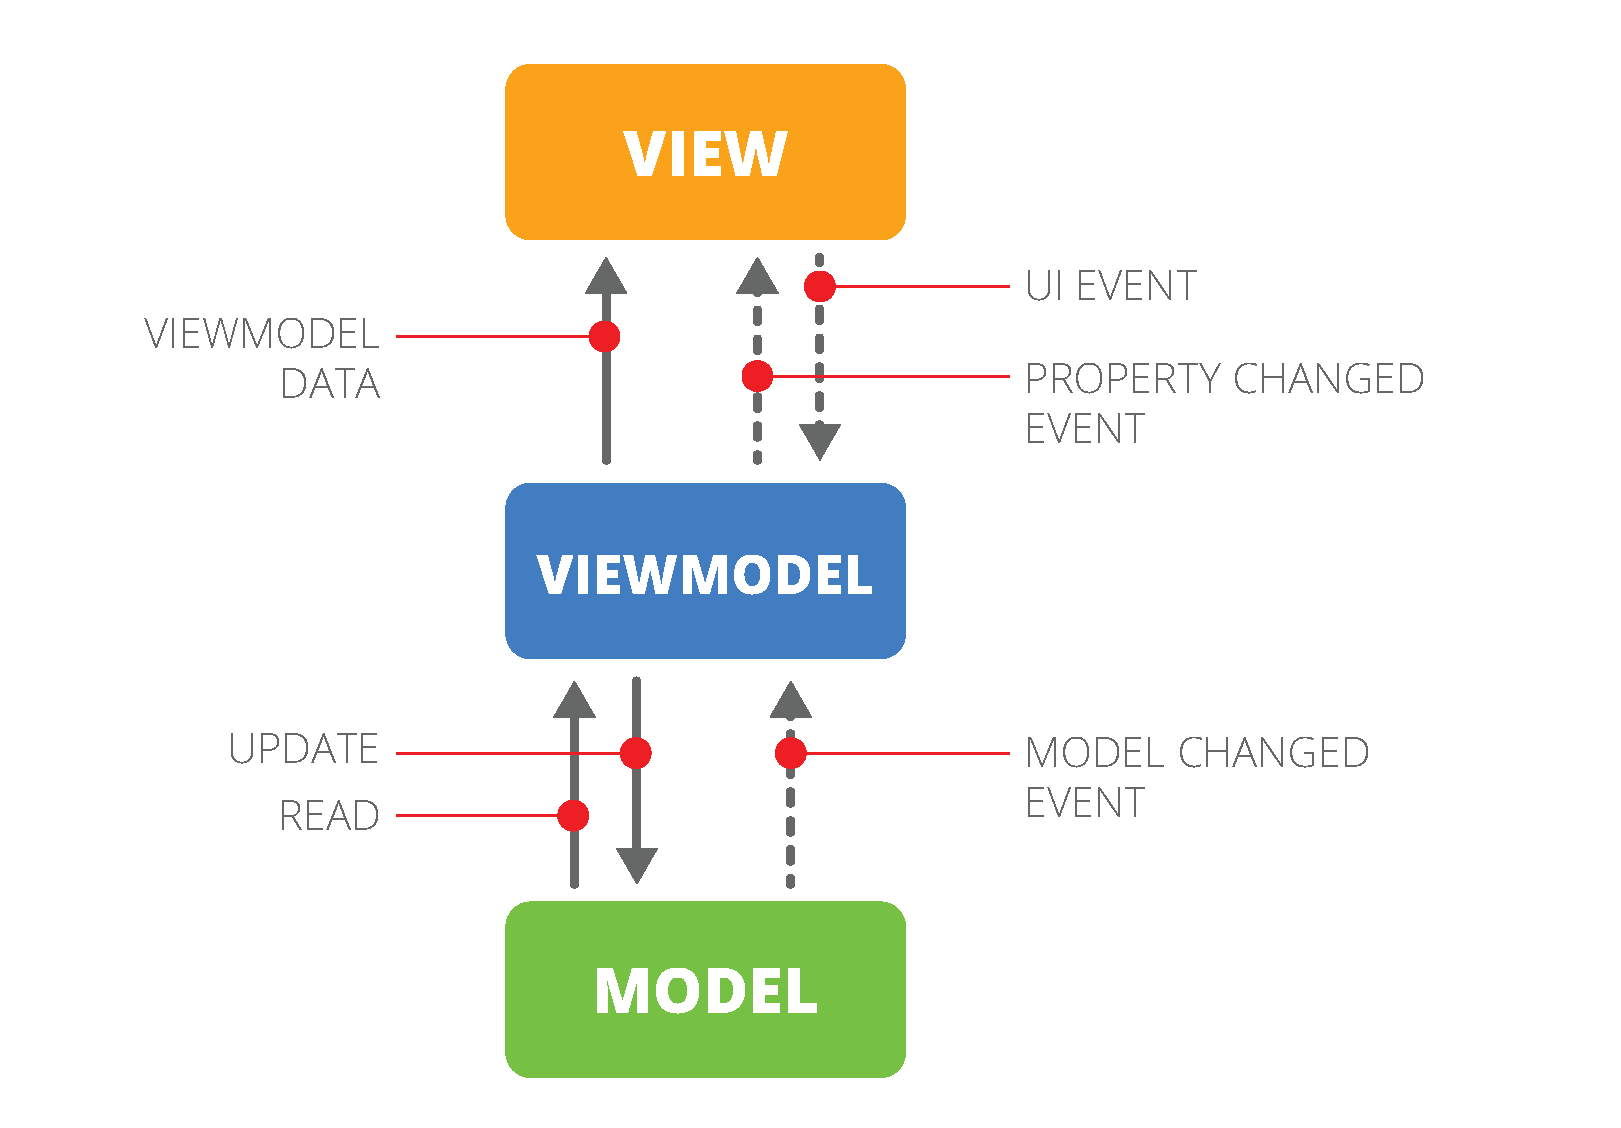
\includegraphics[width=1.0\linewidth]{./img/mvvm}
\caption[Schema delle comunicazioni nel modello MVVM]{Schema delle comunicazioni nel modello MVVM}
\label{fig:mvvvm}
\end{figure}

Questo approccio porta ad avere Model e ViewModel popolati con la maggior parte del codice applicativo, che, di conseguenza, viene rimosso dalla View. Il vantaggio dell'utilizzo dell'MVVM risiede proprio nel fatto che la sezione View, complessa da testare, diventa molto semplice e di fatto � quasi inutile eseguire test sul codice che la genera.

La principale funzionalit� fornita da AngularJS � il \textit{binding} dinamico delle variabili JavaScript con i controlli HTML presenti nella pagina. Il binding � una operazione che permette di collegare una parte di Model con una porzione definita di View. Molto spesso questa funzionalit� � utilizzata per collegare una variabile JavaScript con un controllo HTML, il binding garantisce che quando la variabile assume un nuovo valore, questo sia mostrato sulla interfaccia e, viceversa, quando un utente modifica il valore nella vista, questo venga immediatamente riflesso sulla variabile nel modello. Questo tipo di binding � definito \textit{bidirezionale} o \textit{two-way data binding}.

Il binding � una funzionalit� molto interessante, perch� solleva il programmatore dall'incombenza di mantenere la coerenza tra dati e interfaccia. Automatizzando questa operazione si ottiene anche una semplificazione del codice e una maggiore garanzia di funzionamento dell'applicazione. 

Per implementare il binding bidirezionale, AngularJS si serve di nuovi costrutti che arricchiscono il vocabolario a disposizione del programmatore per la stesura del codice HTML. Segue un esempio di codice contenente i costrutti AngularJS per realizzare un binding.

Contenuto del file \verb|view.html|:
\begin{verbatim}
<!doctype html>
<html ng-app='greetingsApp'>
  <head>
    <script src="angular.min.js"></script>
    <script src="app.js"></script>
  </head>
  <body ng-controller="GreetingsCtrl">
    Hello {{subject}}!
  </body>
</html>
\end{verbatim}

Contenuto del file \verb|app.js|:
\begin{verbatim}
angular.module('greetingsApp', [])
.controller('GreetingsCtrl', function ($scope) {
  $scope.subject = 'World';
});
\end{verbatim}

Esaminando il codice HTML del file view.html nell'esempio, si nota innanzitutto la necessit� di importare libreria JavaScript \verb|angular.min.js| nella pagina web. Questa operazione permette di utilizzare AngularJS all'interno della pagina stessa. Per attivare la libreria all'interno della pagina web �, inoltre, necessario specificare l'attributo \verb|ng-app|. All'applicazione nell'esempio � stato dato nome \verb|greetingsApp|.

AngularJS necessita di uno \textit{scope} nel quale monitorare le variabili che fanno uso del binding. Esso � definito con il l'attributo \verb|ng-controller|. Nell'esempio riportato lo scope sar� esteso a tutto il contenuto del tag \verb|body|. All'interno dello scope, si identificano le variabili della view agganciate al modello con l'utilizzo di una doppia parentesi graffa \verb|{{}}|.

Nell'esempio, la logica dell'applicazione risiede nel file \verb|app.js|, infatti al suo interno � possibile identificare una dichiarazione di controller e una funzione che ne implementa il comportamento. Nel caso riportato il comportamento � molto semplice, si limita all'assegnamento di una variabile utilizzata come modello. 

AngularJS fornisce un insieme piuttosto nutrito di librerie di utilit� che risolvono i pi� comuni problemi di comunicazione con sorgenti esterne di dati. Mole.io utilizza una di queste librerie per mettere in comunicazione i modelli AngularJS con una API REST presente sul server che si occupa di fornire i dati necessari a popolare le variabili. Non appena viene eseguito l'aggiornamento di tali variabili, AngularJS provvede ad aggiornare l'interfaccia utente con i dati ottenuti utilizzando del codice molto simile a quello riportato nell'esempio.

La struttura di questo framework, per sua natura, induce ad un design delle applicazioni per \textit{componenti} indipendenti ma comunicanti. E' possibile infatti immaginare una pagina web contenente diversi costrutti \verb|ng-controller|, ognuno dei quali si occupa di aggiornare una porzione della View con logiche specifiche. Non � difficile comprendere come questo approccio possa favorire la scrittura di software di buona qualit�, attraverso il riuso di componenti e lo studio attento della separazione delle responsabilit� di ogni componente. 

AngularJS utilizza il formato \textit{JavaScript Object Notation} (JSON) per lo scambio di dati tra il backend e i modelli. In \cite{crockford2008javascript} Douglas Crockford illustra questo formato da lui ideato. La definizione di JSON � aderente alle specifiche ECMA-262 del Dicembre 1999, e permette a JavaScript di interpretare questo formato nativamente. JSON quindi � un formato facilmente maneggiabile sia lato frontend, sia lato backend, questo ha contribuito a farlo diventare molto famoso e utilizzato per la realizzazione di applicazioni Node.js.

Per la realizzazione della parte frontend di Mole.io sono state utilizzate diverse librerie JavaScript e framework di supporto alla stesura del codice HTML. Dell'insieme delle librerie utilizzate, si sono estratte le principali, delle quali seguir� una descrizione: 
\begin{itemize}
\item Leaflet
\item D3.js
\item Bootstrap
\end{itemize}

\subsubsection{Leaflet e D3.js}

Uno degli scopi per i quali � stata creata l'applicazione Mole.io � fornire una visione immediata della situazione nella quale le si trovano i sistemi monitorati. Per rendere a \textit{colpo d'occhio} fruibili le informazioni si � pensato di utilizzare mappe geografiche e grafici. Le librerie \textit{leaflet} e \textit{d3.js} hanno rispettivamente questi compiti.\\

\begin{figure}[h]
\centering
\includegraphics[width=0.7\linewidth]{./img/leaflet}
\caption[Il logo di Leaflet]{Il logo di Leaflet}
\label{fig:leaflet}
\end{figure}

\begin{figure}[h]
\centering
\includegraphics[width=0.7\linewidth]{./img/d3}
\caption[Il logo di D3.js]{Il logo di D3.js}
\label{fig:d3}
\end{figure}

\begin{description}
\item[leaflet] \cite{website:Leaflet} � una libreria JavaScript che si occupa di gestire e mostrare a video mappe geografiche. La principale particolarit� di questo software � il fungere da \textit{layer di astrazione} rispetto ai vari sistemi per la gestione di mappe geografiche esistenti. L'utilizzo di plugin, infatti, permette a leaflet di interfacciarsi con svariati \textit{provider} di mappe online tra i quali Google Maps, CloudMade, OpenStreetMap, Esri e Nokia.
Questa libreria offre molte funzionalit� per interagire con le mappe caricate; tra le principali, la possibilit� di utilizzare \textit{overlay}, per evidenziare specifiche aree o porzioni di territorio e \textit{marker} per indicare punti specifici nella mappa. \`{E} possibile, inoltre, arricchire i marker con testo e immagini caricabili quando l'utente clicca sull'icona del marker stesso. Uno dei principali motivi che hanno contribuito alla scelta di leaflet come libreria per rappresentare mappe, � l'aspetto della compatibilit� con i diversi browser. Questa libreria infatti garantisce un alto grado di compatibilit� con i principali browser per desktop e \textit{smartphone}.  

\begin{figure}[h]
\centering
\includegraphics[width=0.7\linewidth]{./img/leaflet-map}
\caption[Un esempio di mappa realizzata con Leaflet]{Un esempio di mappa realizzata con Leaflet}
\label{fig:leaflet-map}
\end{figure}

\item[d3.js] \cite{website:D3.js} il nome di questa libreria significa \textit{Data-Driven Documents} e ne riassume perfettamente le funzionalit�. Essa permette, infatti, di generare grafici e documenti a partire da \textit{set} di dati. Come Leaflet, anche D3 � altamente compatibile con i diversi browser, in quanto i grafici sono prodotti utilizzando i linguaggi HTML o SVG. L'SVG � un linguaggio derivato da XML che offre costrutti in grado di rappresentare grafiche \textit{raster} e \textit{vettoriali}. L'uso di queste tecnologie largamente diffuse all'interno dei diversi browser permette a D3 di garantire una discreta compatibilit� \textit{cross-browser}.

\begin{figure}[h]
\centering
\includegraphics[width=0.7\linewidth]{./img/d3-graph}
\caption[Un esempio di grafico realizzato con D3.js]{Un esempio di grafico realizzato con D3.js}
\label{fig:d3-graph}
\end{figure}

\end{description}

\subsubsection{Bootstrap}

Questa libreria merita una trattazione separata, in quanto non si occupa, come le precedenti, di risolvere in modo specifico un singolo problema, come nel caso della gestione delle mappe o dei grafici, bens� il suo campo di applicazione � molto pi� vasto.

Bootstrap \cite{website:Bootstrap} � infatti una collezione di strumenti che cooperano per fornire allo sviluppatore una piattaforma di templating CSS e JavaScript per la costruzione di moderne pagine web. Essa contiene set, con design preconfigurati, di componenti come bottoni, form, elementi per la navigazione e tipografici.

Seguendo semplici regole di stesura del codice HTML, anche uno sviluppatore con scarsa conoscenza del linguaggio CSS e scarse nozioni di design, � in grado di creare pagine web completamente stilizzate e funzionanti in pochissimo tempo. 

L'idea alla base di Bootstrap � la standardizzazione di pattern di sviluppo e di design utilizzati nella realizzazione di applicazioni web. L'utilizzo di questo framework, infatti, ne velocizza e semplifica molto lo sviluppo.

Tra le principali funzionalit� e le caratteristiche che hanno reso Bootstrap famoso e utilizzato da moltissimi sviluppatori, troviamo:
\begin{itemize}
\item compatibilit� con i maggiori browser
\item \textit{gracefully-degrade} se usato su browser pi� datati
\item supporto del design responsivo
\item adattamento a diversi dispositivi (desktop, smartphone, tablet)
\item licenza open source
\item struttura modulare ed estensibile
\end{itemize}
	\clearpage
		\subsection{Gestione delle dipendenze}\label{Gestione_delle_dipendenze}
		\clearpage
	\section{Strumenti per il deploy}\label{Strumenti_per_il_deploy}
	\clearpage

\chapter{Mole.io}\label{Moleio}
	In questo capitolo descriveremo nel dettaglio Mole.io: un nuovo sistema per la gestione centralizzata dei log, realizzato come progetto di questa tesi.

Iniziamo immediatamente con la doverosa spiegazione dell'origine del nome di questo software.

\textit{Mole} � una parola inglese che significa \textit{talpa}. Nel gergo dello spionaggio, la talpa, � un infiltrato che viene inserito in un sistema avversario e cattura informazioni che riferisce all'\textit{intelligence} della sua fazione.   

Il nostro sistema, si comporta esattamente come un infiltrato: passa informazioni del sistema nel quale viene inserito, le applicazioni da monitorare, alla sua organizzazione, gli sviluppatori.

Ogni talpa che si rispetti ha alcuni contatti all'interno del sistema che gli riportano le informazioni rilevanti. Abbiamo chiamato questi contatti \textit{mole-contacts} e le soffiate da loro riferite \textit{whispers}.

Nel nostro sistema, i \textit{mole-contacts} sono moduli software che risiedono all'interno dell'applicazione da monitorare, catturano le situazioni significative per il software nel quale operano ed inviano degli \textit{whisper} ad un server chiamato \textit{mole}.

Nell'immaginario collettivo l'infiltrato � una persona ben vestita, con un abito elegante, giacca, cravatta e cappello. Anche il nostro software, in un certo senso, � ben vestito, infatti possiede una interfaccia grafica realizzata per monitorare le applicazioni ed organizzare gli whisper in arrivo. Questo componente si chiama \textit{mole-suit}.\\

Il progetto al momento � un prototipo, ma il � destinato ad essere ultimato per diventare un servizio vero e proprio fornito via web. in figura \ref{fig:mole-logo} � riportato il logo proposto per Mole.io.\\

\begin{figure}[h]
\centering
\includegraphics[width=0.7\linewidth]{./img/mole-logo}
\caption[Il logo di Mole.io]{Il logo di Mole.io}
\label{fig:mole-logo}
\end{figure}

Nella sezione seguente vedremo quali sono le funzionalit� specifiche di ogni componente in Mole.io, con particolare attenzione al modo nel quale tali componenti scambiano dati tra loro.


	\clearpage
	\section{Architettura del sistema}\label{Architettura_del_sistema}
		Come abbiamo anticipato nell'introduzione di questo capitolo, Mole.io � organizzato in diverse componenti, ognuna delle quali possiede un compito specifico e interagisce con altre.

Nell'architettura di Mole.io si possono innanzitutto individuare due macro-componenti principali. Nelle sezioni seguenti ne illustreremo la struttura.

%TODO parlare di REST

\subsubsection{Insertion}

Questo \textit{layer} dell'applicazione si occupa dell'inserimento dei dati nel sistema e si avvale di diversi moduli per fare in modo che gli whisper vengano salvati, aggregati e organizzati nel database.

Nello schema \ref{} � riportata l'architettura del layer di insertion, essa � composta da diversi moduli:

mole-contacts

la porzione di sistema che si occupa dell'inserimento dei dati provenienti dall'esterno, � composta a sua volta dai \textit{mole-contacts}, da \textit{mole} e dai \textit{denormalizers}.



\begin{description}
\item [insertion] � la porzione di sistema che si occupa dell'inserimento dei dati provenienti dall'esterno, � composta a sua volta dai \textit{mole-contacts}, da \textit{mole} e dai \textit{denormalizers}.
\item [presentation] si occupa dell'estrazione dei dati dal sistema e della loro presentazione all'utente. 
\end{description}


% dire che esistono 2 server
% dire che la ui � separata e statica e pu� essere servita da un terzo server
% configurazione rabbit utilizzata per scalare (broadcast+loadbalancing)

% middleware
		\clearpage
		\subsection{CQRS ed estensibilit�}\label{CQRS_ed_estensibilita}
		%TODO
% cosa è CQRS
% come Mole.io implementa il pattern

% preblema del read/write lock di mongo (qui o sulla scalabilità?)

		\clearpage
		\subsection{mole}\label{mole}
			\subsubsection{I denormalizzatori}\label{I_denormalizzatori}
			\clearpage
		\subsection{mole-suit}\label{mole-suit}
			\subsubsection{I plugin e gli widget}\label{I_plugin_e_gli_widget}
			\clearpage
	\section{Autenticazione degli utenti}\label{Autenticazione_degli_utenti}
	\clearpage
	\section{Scalabilit� e affidabilit�}\label{Scalabilita_e_affidabilita}
	\clearpage
	\section{Problematiche di sviluppo}\label{Problematiche_di_sviluppo}
	\clearpage

\chapter{Configurazioni e benchmark}\label{Configurazioni_e_benchmark}
I test eseguiti su Mole.io hanno privilegiato l'aspetto della raccolta dati operata dal sistema. Questa, infatti, � una delle principali funzionalit� offerte dall'applicazione ed � interessante comprendere come, l'ottimizzazione del layer di insert, possa contribuire ad un incremento delle performance globali del sistema.

Durante i test sono state esplorate diverse configurazioni del database al fine di comprendere quale fosse la ottimale ai fini applicativi per Mole.io. I test sono stati eseguiti cercando di creare un ambiente il pi� possibile esente da fattori di incertezza esterni, al fine ottenere misure affidabili e risultati riproducibili.

Per lo svolgimento delle analisi, � stato realizzato un cluster MongoDB utilizzando tre \textit{virtual machine} (VM) rispettivamente configurate in modo da utilizzare 512 Mb di memoria RAM, con un Hard Disk SSD da 8,0 Gb e dotate di un processore da 1,2 GHz. Ognuna delle VM � stata equipaggiata con una differente configurazione:
\begin{description}
\item[VM1] sulla quale sono stati installati un Query Router (\verb|mongos|), il cui compito � stato fornire l'accesso all'intero cluster e un Config Server (\verb|mongod|) opportunamente configurato per tenere traccia delle informazioni di \textit{layout} del cluster;
\item[VM2] su cui � stato installato il primo shard utilizzando un demone \verb|mongod|;
\item[VM3] clone della macchina precedente, necessaria per il secondo shard del cluster;
\end{description}

I test sono stati svolti utilizzando diverse configurazioni del cluster realizzato e misurando i tempi per l'inserimento di dati nel database. Per comprendere il significato delle diverse configurazioni del cluster, � necessario fare riferimento ad una nota, relativa alle chiavi di sharding, all'interno della documentazione di MongoDB:

\begin{quote}
\textit{When inserting documents with monotonically increasing shard keys, all inserts belong to the same chunk on a single shard. The system will eventually divide the chunk range that receives all write operations and migrate its contents to distribute data more evenly. However, at any moment the cluster can direct insert operations only to a single shard, which creates an insert throughput bottleneck.}
\end{quote}

Un requisito fondamentale di una buona chiave di sharding in MongoDB � la distribuzione probabilistica dei suoi valori. La documentazione di MongoDB, infatti, consiglia di utilizzare chiavi con una distribuzione di valori il pi� uniforme possibile, in modo da mantenere costante il carico di lavoro assegnato ad ogni shard. Da questo punto di vista, una buona chiave di sharding � l'id fornito automaticamente da MongoDB ad ogni documento.

Come � possibile leggere dalla citazione tratta dalla documentazione del database, per�, � fondamentale che le chiavi di sharding non utilizzino valori  monotoni, pena una riduzione significativa delle performance. Questo � dovuto al fatto che il balancer di MongoDB utilizza una logica di partizionamento basata sui valori delle chiavi. In presenza di valori con distribuzione monotona, il balancer non � in grado di eseguire un bilanciamento in tempo reale dei valori, e li salva sempre nell'ultimo shard disponibile, degradando le performance dell'intero cluster. L'\textit{id} fornito da MongoDB � generato a partire da un \textit{timestamp}, quindi, per costruzione, i valori degli id sono monotonicamente crescenti.

A fronte delle considerazioni precedenti, � stato scelto di eseguire i test utilizzando configurazioni del cluster differenziate sulla base della chiave di sharding scelta per bilanciare la base dati:
\begin{enumerate}
\item un solo shard, nessuna chiave di sharding;
\item due shard, utilizzando come chiave di sharding il campo \textit{id} fornito da MongoDB;
\item due shard, utilizzando come chiave il valore \textit{hash} del campo id, questo permette di ottenere, contemporaneamente, valori con distribuzione uniforme, non monotonicamente crescenti.
\end{enumerate}

I valori raccolti durante i test si riferiscono al tempo richiesto per inserire un numero definito di documenti all'interno del cluster. Sono stati utilizzati due tipi di documenti: \textit{small}, della dimensione di 200 byte circa, e \textit{big}, con una dimensione pari a 1 Megabyte. 

Per verificare la risposta del sistema al crescere del carico di lavoro richiesto, � stato creato uno script in grado di simulare un numero variabile di client (\textit{thread}). Ogni client esegue un numero prefissato di richieste di inserimento all'interno del database. 

Il numero dei client � stato fatto variare progressivamente da 1 a 100 con incrementi di 10. Il numero di richieste per client � stato impostato a 10 per i documenti di tipo \textit{big} e a 100 per i documenti di tipo \textit{small}. 

Le tabelle \ref{tab:benchmark-small} e \ref{tab:benchmark-big} riportano i risultati ottenuti, rispettivamente per i test eseguiti utilizzando documenti di tipo \textit{small} e \textit{big}. I valori riportati in tabella sono la media dei valori ottenuti da tre esecuzioni. I grafici \ref{fig:benchmark-small} e \ref{fig:benchmark-big} sono stati ottenuti ponendo sull'asse delle ascisse il numero dei client, e sull'asse delle ordinate il tempo richiesto dal cluster per l'inserimento di tutti i documenti del test.\\

\begin{table}[h]
\begin{center}
\begin{tabular}{r||r|r|r}
Client & 1 Shard & 2 Shard (id) & 2 Shard (hashed id) \\ 
\hline \hline 
1 & 0.239 & 0.172 & 0.285 \\
10 & 0.451 & 0.442 & 0.448 \\
20 & 0.884 & 0.909 & 0.983 \\
30 & 1.310 & 1.395 & 1.460 \\
40 & 1.776 & 1.859 & 1.960 \\
50 & 2.281 & 2.319 & 2.525 \\
60 & 2.751 & 2.862 & 3.112 \\
70 & 3.275 & 3.484 & 3.925 \\
80 & 3.798 & 3.910 & 4.525 \\
90 & 4.201 & 4.358 & 4.856 \\
100 & 4.784 & 4.967 & 5.604 \\
\end{tabular}
\caption{Risultati dei test con documenti \textit{small}}\label{tab:benchmark-small}
\end{center}
\end{table}

\begin{figure}[h]
\centering
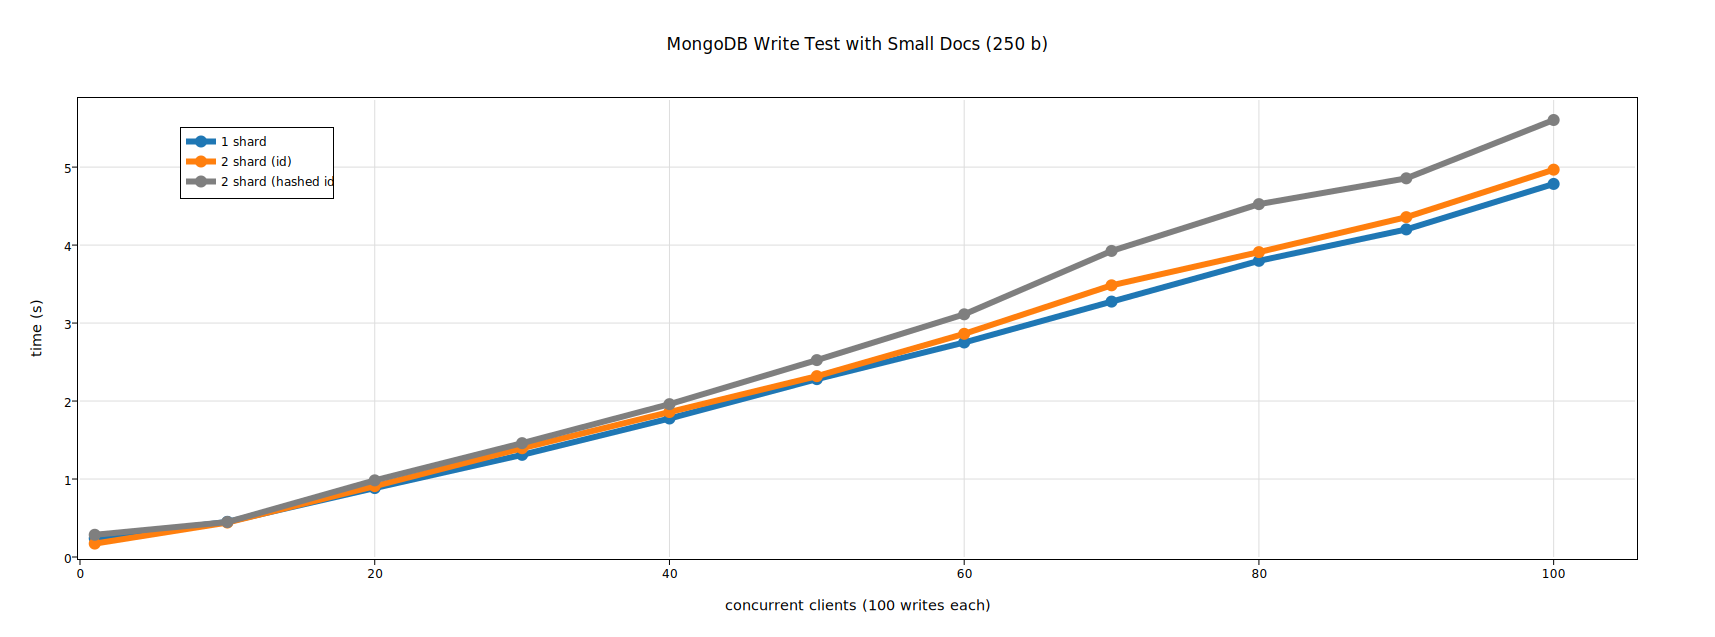
\includegraphics[width=1.0\linewidth]{./img/mongodb_write_test_with_small_docs_250_b}
\caption[Grafico dei risultati con documenti \textit{small}]{Grafico dei risultati con documenti \textit{small}}
\label{fig:benchmark-small}
\end{figure}

\begin{table}[h]
\begin{center}
\begin{tabular}{r||r|r|r}
Client & 1 Shard & 2 Shard (id) & 2 Shard (hashed id) \\ 
\hline \hline 
1 & 0.682 & 0.828 & 0.692 \\
10 & 2.165 & 2.853 & 2.095 \\
20 & 7.009 & 7.243 & 4.290 \\
30 & 8.753 & 10.141 & 6.335 \\
40 & 14.535 & 15.912 & 9.089 \\
50 & 31.931 & 43.645 & 12.949 \\
60 & 30.808 & 24.503 & 15.000 \\
70 & 46.350 & 59.534 & 19.179 \\
80 & 32.045 & 43.703 & 28.898 \\
90 & 114.287 & 97.787 & 25.843 \\
100 & 127.658 & 88.600 & 32.171 \\
\end{tabular}
\caption{Risultati dei test con documenti \textit{big}}\label{tab:benchmark-big}
\end{center}
\end{table}

\begin{figure}[h]
\centering
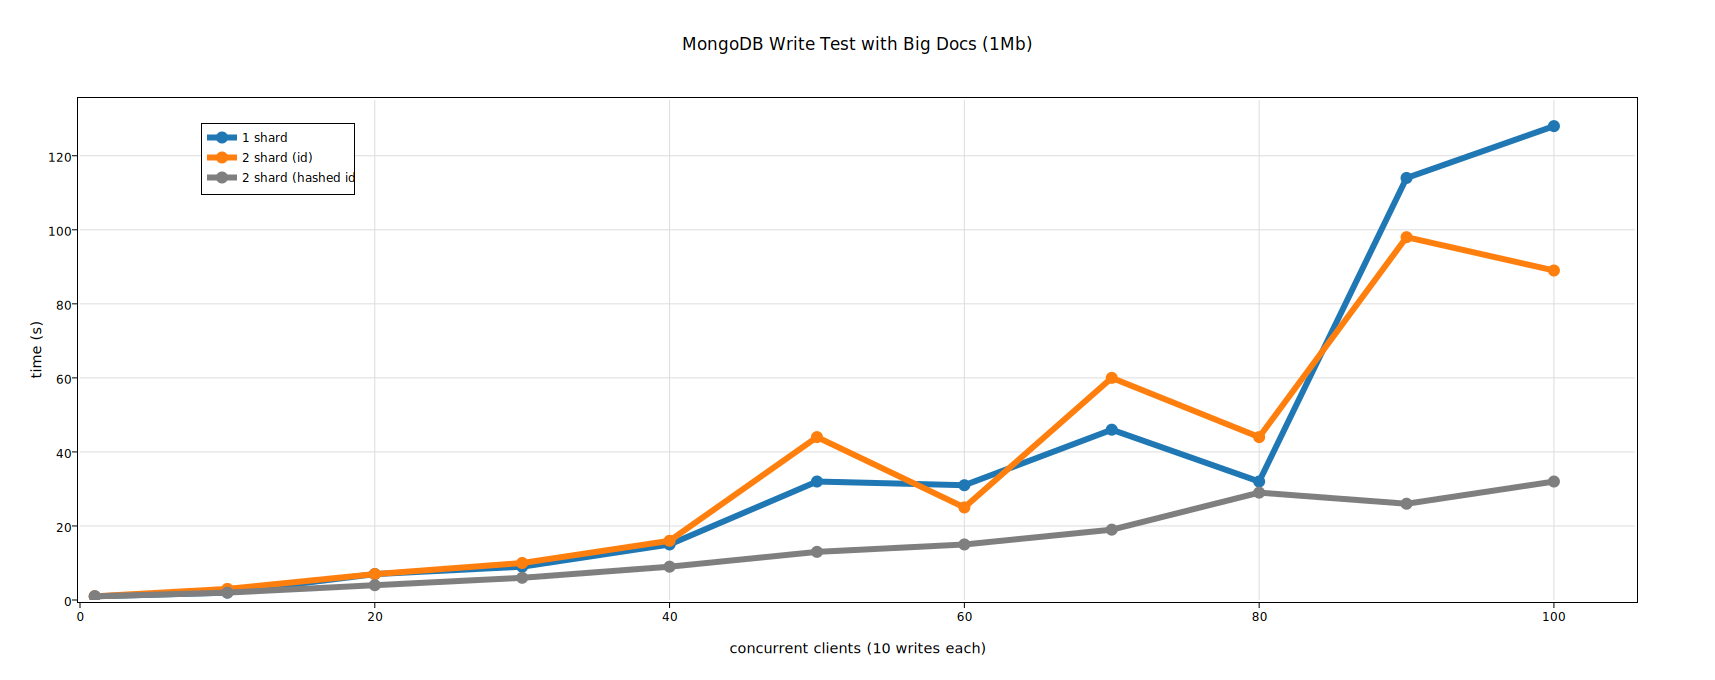
\includegraphics[width=1.0\linewidth]{./img/mongodb_write_test_with_big_docs_1mb}
\caption[Grafico dei risultati con documenti \textit{big}]{Grafico dei risultati con documenti \textit{big}}
\label{fig:benchmark-big}
\end{figure}

Osservando i risultati ottenuti � chiaro come lo sharding offra vantaggi concreti solo se la dimensione dei documenti da salvare � consistente. Il motivo di questo comportamento, risiede nella modalit� di lavoro del balancer e nella politica di gestione dei lock applicata da MongoDB.

Salvando documenti di piccole dimensioni su pi� shard, accade che il tempo richiesto dal write-lock � minimo e, di conseguenza non si arriva alla \textit{saturazione} delle code di scrittura del database. Scegliendo la politica di sharding che fa uso di hash, inoltre, il balancer � obbligato ad eseguire uno spostamento dei documenti a \textit{runtime}, degradando le performance rispetto alla scrittura su un singolo shard.

Nel caso di documenti di dimensioni maggiori, invece, l'\textit{overhead} aggiunto dal balancer � minimo rispetto al tempo di attesa dei documenti sulla coda di scrittura. Come conseguenza, si ottiene che l'utilizzo di pi� shard, e quindi di pi� code di scrittura parallele, aumenta notevolmente le performance dell'intero cluster.
\clearpage

\chapter*{Conclusioni e sviluppi futuri\markboth{}{Conclusioni e sviluppi futuri}}\label{Conclusioni_e_sviluppi_futuri}
\addcontentsline{toc}{chapter}{Conclusioni e sviluppi futuri}
La realizzazione di un sistema come Mole.io ha permesso di ottenere una ottima visione generale delle possibilit� offerte dai moderni strumenti per la costruzione di applicazioni web. I diversi \textit{tool} a disposizione permettono infatti di realizzare in breve tempo applicazioni complete, stabili e flessibili, in grado di scalare facilmente su sistemi PaaS.

Riuscire ad ottenere una ambiente di test ottimale, esente, per quanto possibile da fattori esterni, si � rivelata una operazione difficoltosa. Il numero di variabili che concorrono alla riuscita di un singolo test �, infatti, consistente. \`{E} necessario, ad esempio, tenere in considerazione eventuali latenze legate all'infrastruttura di rete (reale o virtuale), parametri di configurazione specifici dei sistemi operativi nei quali i diversi applicativi vengono eseguiti, nonch� eventuali problematiche legate agli ambienti di virtualizzazione utilizzati.

I test eseguiti hanno mostrato caratteristiche salienti di MongoDB e problematiche importanti legate a questo database. I nuovi test dovranno concentrarsi principalmente sul layer di presentation, per comprendere come ottimizzare la configurazione del database al fine di massimizzare il throughput del sistema nel caso dell'estrazione dei dati. Nell'immediato futuro, quindi, sar� necessario eseguire ulteriori analisi per comprendere se questa tecnologia sia quella ottimale per l'ambito applicativo di Mole.io, oppure si rendano necessarie particolari configurazioni o alternative a MongoDB. 

Durante lo sviluppo di Mole.io sono state proposte diverse funzionalit� del sistema, alcune delle quali sono state implementate nel prototipo iniziale realizzato per questa tesi. Molte idee, per�, sono rimaste irrealizzate. Di seguito, quindi, un elenco delle funzionalit� interessanti da sviluppare in futuro su Mole.io:
\begin{description}
\item[Nuovi mole-contact] l'implementazione di nuovi mole-contact, necessari per coprire buona parte dei linguaggi utilizzati per lo sviluppo di applicazioni web, mobile e desktop;
\item[HTTPS] utilizzo di un protocollo HTTP Secure per lo scambio delle comunicazioni, in modo da garantire un alto livello di sicurezza agli utenti;
\item[Archiviazione dei vecchi whisper] in modo da mantenere all'interno dell'interfaccia utente solo le informazioni utili per la comprensione dello stato della source in esame;
\item[Nuovi denormalizzatori] lo sviluppo di denormalizzatori, plugin e widget per la gestioni di nuove tipologie di dati, in modo da fornire un \textit{set} di strumenti completo e funzionale per utenti e sviluppatori;
\item[Notifiche push] la possibilit�, cio�, di aggiornare in tempo reale le pagine visualizzate dall'utente inviando i nuovi dati ottenuti dalle source;
\item[App mobile] la realizzazione di una applicazione \textit{mobile} per la consultazione dello stato delle source e la ricezione, su smartphone, di eventuali avvisi in caso di malfunzionamenti del sistema;
\item[Linguaggio di query] l'implementazione di un linguaggio di query, con una interfaccia utente appositamente studiata, per rendere facile la visualizzazione dei dati raccolti in maniera aggregata e filtrata;
\end{description}

\clearpage

\bibliography{Bibliografia}
\bibliographystyle{unsrt}
\addcontentsline{toc}{chapter}{Bibliografia}

\end{document}

%
%il problema
%- problema del logging:
%  - tante applicazioni
%  - diversi clienti
%  - report errori
%
%stato dell'arte: i software di logging centralizzato
%- aircoso
%- fluentd + elastic search + kibana
%perch\'{e} lo stato dell'arte non ci piace
%- non permettono di avere "modelli/template di messaggi" flessibili
%- contesti differenti
%
%il nostro logger 
%- perch\'{e} abbiamo scelto nodejs
%- cos'� nodejs (storia, peculiarit�, async, pesca da presentazione lucio)
%- come funziona il logger (struttura e schema delle comunicazioni di rete)
%- problematiche incontrate durante l'implementazione
%- si auto-adatta al tipo di messaggio in arrivo
%- denormalizzatori
%- plugin/widget
%- il clAud
%- architettura del sistema
%- estensibilit�
%- come scrivere plugin e widget
%
%problematiche "accademiche"
%- sicurezza (oauth)
%- scalabilit� (+ server con load balancer? cloud? rabbit, disaccoppiamento dei servizi)
%- relayability (+ server ridondati) 
%
%
%
%Scaletta:
%
%Metodologie:
% - CQRS
% - TDD
% - user stories
%
%Tecnologie utilizzate:
%- NodeJS
%  - npm (gestione dipendenze)
%  - passport (oauth)
%  - mongoskin
%  - mongoose
%  - underscore
%  - express
%  - faker (fixtures)
%  - grunt (automation)
%  - mocha (testing)
%  - should (testing)
%  - supertest (testing)
%  - require-all (plugin)
%  - cors (e problemi correlati)
%
%- rabbitmq
%
%- angularjs
%  - leflet (mappe)
%  - directive
%  - controller
%  - views
%  - services
%  - filters
%  - karma (testing)
%  - d3 (grafici)
%  - jquery
%  - bootstrap (ui)
%  - bower (gestione dipendenze)
%
%- mongodb
%  - sharding
%  - replicaset
%
%- dokku
%  
%- git(?)





